\documentclass{beamer}
\usetheme{CambridgeUS}
\usefonttheme{serif}
\usecolortheme{dove}
\useinnertheme{rounded}
%\useoutertheme{miniframes}
\usepackage{graphicx}
\usepackage{setspace}
\usepackage{tabularx}
\usepackage{tikzsymbols}
\usepackage{tikz}
\usepackage{spot}
\usepackage[italian]{babel}
\usepackage{tabularx}
\usepackage[absolute,overlay]{textpos}
\usepackage{booktabs}
\usepackage{fancyvrb}
\usepackage{xcolor}
\usepackage{multicol}
\usepackage{multirow}


\newcommand\Factor{1.2}
\definecolor{unipd}{RGB}{155, 0, 20}
\definecolor{grigioPantano}{RGB}{72,79,89}


\setbeamerfont{block title}{family=\bfseries}
\setbeamercolor{block title}{use=structure,fg=unipd,bg=white}

%\setbeamertemplate{footline}[page number]
\setbeamerfont{subtitle}{size=\large, series=\bfseries}
\definecolor{template}{RGB}{54, 114, 89}
\definecolor{background}{RGB}{250, 250, 250}
\definecolor{royalblue3}{RGB}{58,95,205}
\definecolor{giallo}{RGB}{197, 151, 0}
\definecolor{blu}{RGB}{19 101 158}
\setbeamercolor{frametitle}{fg=template, bg=white}
\setbeamercolor{section in head/foot}{bg=template, fg=template!20}
\setbeamercolor{subsection in head/foot}{bg=template!20, fg=template}
\setbeamercolor{author in head/foot}{bg=template, fg=template!20}
\setbeamercolor{date in head/foot}{bg=template, fg=white}
\setbeamercolor{page number in head/foot}{bg=template, fg=white}
\setbeamercolor{title in head/foot}{fg=template}
\setbeamercolor*{item}{fg=template}
\setbeamertemplate{frametitle}{\color{template}\bfseries\scshape\insertframetitle\par\hrulefill}
\setbeamercolor{title}{fg=template}
\definecolor{unipd}{RGB}{155, 0, 20}
\definecolor{highlight}{RGB}{54, 114, 89}
\definecolor{back}{RGB}{247, 251, 255}
\definecolor{map}{RGB}{111, 172, 232}
\definecolor{childmap}{RGB}{161, 200, 240}
\definecolor{nodemap}{RGB}{141, 170, 199}
\definecolor{rasch}{rgb}{0.0, 0.33, 0.71}
\definecolor{log}{rgb}{0.0, 0.65, 0.58}
\definecolor{diff}{RGB}{33, 113, 181}
\definecolor{single}{RGB}{106, 81, 163}
\definecolor{comp}{RGB}{35, 99, 70}
\definecolor{inc}{RGB}{191, 13, 43}
\definecolor{highlight}{rgb}{0.45, 0.31, 0.59}
\definecolor{section}{RGB}{51,51,179}
\definecolor{typical}{RGB}{8, 69, 148}
\definecolor{model}{RGB}{74, 20, 134}
\definecolor{orangered2}{RGB}{238,64,0}
\definecolor{royalblue3}{RGB}{58,95,205}
\definecolor{springgreen}{RGB}{0,205,102}
\definecolor{magenta}{RGB}{255,0,255}

  \tikzset{
	invisible/.style={opacity=0},
	visible on/.style={alt={#1{}{invisible}}},
	alt/.code args={<#1>#2#3}{%
		\alt<#1>{\pgfkeysalso{#2}}{\pgfkeysalso{#3}} % \pgfkeysalso doesn't change the path
	},
	every overlay node/.style={
		%draw=black,fill=white,rounded corners,
		anchor=north west, inner sep=0pt,
	},
}

\usetikzlibrary{shapes.geometric, arrows}
\tikzstyle{respondent} = [rectangle, minimum width=1.5cm, minimum height=1cm,text centered, draw=white]
\tikzstyle{stimulus} = [rectangle, minimum width=1.5cm, minimum height=1cm,text centered, draw=white]
\tikzstyle{trial} = [rectangle, minimum width=1cm, minimum height=1cm,text centered, draw=black]
\tikzstyle{process} = [rectangle, rounded corners, minimum width=0.5cm, minimum height=1cm, text width =2.5cm, text centered, draw=black]
\tikzstyle{arrow} = [thick,->,>=stealth]
\tikzstyle{condition} = [rectangle, rounded corners,draw=black,text width=2cm, text height=6.5cm]
\tikzstyle{latent} = [ellipse, minimum width=2.5cm, minimum height=2cm,text centered, draw=black]
\tikzstyle{item} = [rectangle, rounded corners, minimum width=0.5cm, minimum height=1cm, text width =1.5cm, text centered, draw=black]
\tikzstyle{arrow} = [thick,->,>=stealth]

\def\tikzoverlay{%
	\tikz[remember picture, overlay]\node[every overlay node]
}%


\AtBeginSection[]
{
	\begin{frame}
		\tableofcontents[currentsection,currentsubsection]
	\end{frame}
}  



%\title[Implicit assessment]{Implicit assessment in psychology: \\ How to work with the IAT}
\title[Misurazione implicita]{Misurazione Implicita in Psicologia: \\ Definizioni, critiche ed evoluzioni}
\date[PSQT, 2024]{Master di II Livello \\ Psicologia quantitativa: Misurazione, valutazione e analisi di variabili psicosociali }
\institute[]{18 luglio 2024, Padova}
\author[Ottavia M. Epifania]{\texorpdfstring{Ottavia M. Epifania, Ph.D.\newline\url{ottavia.epifania@unipd.it}}{Author}}

\begin{document}
	\tikzstyle{every picture}+=[remember picture]
	


\begin{frame}[plain]
    \maketitle
\end{frame}


\section{Cognizione e Cognizione sociale}


\begin{frame}
	\begin{itemize}
		\item \textbf{Cognition}: mental action or process of acquiring knowledge and understanding through thought, experience, and the senses (Oxford University Press, 2020)
		\pause
		\item  \textbf{Social Cognition}:  refers to the processes by which
		people come to understand others (Schacter, Gilbert, \& Wegner, 2009
		\pause
		\item \textbf{Implicit Social Cognition}: cognitive processes that occur outside conscious awareness or conscious control in relation to social psychological constructs: attitudes, stereotypes, and self-concepts (Greenwald \& Banajii, 1995)
	\end{itemize}
\end{frame}


\begin{frame}{Categorizzare}
	
	\begin{columns}[T]
		\begin{column}{.50\linewidth}
			\begin{block}{Cognizione}
				
				Uno stimolo viene identificato come membro di una determinata categoria (ovvero, una classe di stimoli correlati, che hanno qualcosa in comune) 
				
				\begin{figure}
					\centering
					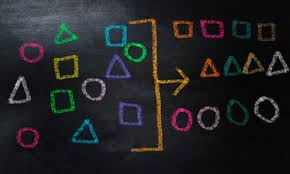
\includegraphics[width=0.3\linewidth]{categorize}
				\end{figure}
				
			\end{block}
		\end{column}
		\begin{column}{.50\linewidth}
			\begin{block}{Cognizione sociale}
				
				Anche le persone vengono categorizzate $\rightarrow$ In base alle categorie di appartenenza si fanno inferenze sulle singole persone 
				
				\begin{figure}
					\centering
					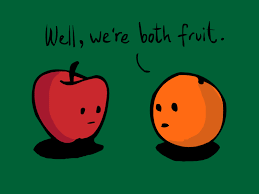
\includegraphics[width=0.3\linewidth]{categorize1}
				\end{figure}
				
			\end{block}
			
		\end{column}
	\end{columns}
\end{frame}


\section[Validità delle misure]{Validità delle misure in Psicologia}

\begin{frame}
	
	\begin{block}{Validità di costrutto}
		
		Quello che si sta misurando... è proprio quello che si voleva misurare e non altro!
		
		(Alcuni) Elementi utili per la \underline{validità di costrutto}:
		\begin{itemize}
			\item Chiara definizione del costrutto teorico
			\item Misurare il costrutto con metodi differenti
		\end{itemize} 
	\end{block}	
	
	\pause
	\begin{block}{Validità statistica}
		
		Quello che stiamo inferendo a partire dalle analisi ha senso perché le analisi hanno senso! 
		
		(Alcuni) Elementi utili per la \underline{validità statistica}:
		\begin{itemize}
			\item Appropriatezza dei metodi statistici utilizzati sulla base delle variabili misurate
			\item Adeguatezza dell'ampiezza campionaria
		\end{itemize} 
		
	\end{block}
\end{frame}


\section[Misurazione esplicita]{Misurazione esplicita}

\begin{frame}
	Il processo di misurazione è \textbf{esplicito}, nel senso che alla persona viene chiesto direttamente di riportare i propri vissuti.
	
	\begin{exampleblock}{}
		
		\begin{itemize}
			\item Quanto sei d'accordo con l'affermazione ``Sono una persona puntuale''
			\item Con quale frequenza ti sei sentito allegro nelle due ultime due settimane? 
			\item Quanto ti ritieni soddisfatto del corso di statistica? 
			\item Ti piacciono i fiori?
		\end{itemize}
	\end{exampleblock}
\end{frame}

\begin{frame}{Item Vero/Falso}
	Sono item formulati in modo che l'unica possibile risposta possa essere Sì/No o Vero/Falso 
	
	\begin{quote}{Esempio}
		
		Mi commuovo quando vedo un film drammatico.
		\begin{itemize}
			\item[$\square$] Sì
			\item[$\square$] No
		\end{itemize}
	\end{quote}
	
	\begin{exampleblock}{Vantaggi}
		
		Sono estremamente facili da comprendere per chiunque 
	\end{exampleblock}
	
	\begin{alertblock}{Svantaggi}
		
		La scala di risposta potrebbe essere troppa riduttiva e particolarmente complessa per certe tipologie di persone
	\end{alertblock}
\end{frame}

\begin{frame}{Risolvere il problema(?)}
	Aggiunta di un terzo punto, ad esempio ``Non so'', ``A volte'', ``Dipende'' ecc.: 
	
	\begin{quote}
		Mi commuovo quando vedo un film drammatico
	\end{quote}
	

	\begin{columns}[T]
		\begin{column}{.50\linewidth}
			\begin{enumerate}
				\item[$\square$] Sì
				\item[$\square$] No 
				\item[$\square$] A volte
			\end{enumerate}
		\end{column}

		\begin{column}{.50\linewidth}
			\begin{enumerate}
				\item[$\square$] Sì
				\item[$\square$] A volte
				\item[$\square$] No
			\end{enumerate}
		\end{column}
	\end{columns}
	\vspace{1.5mm}
	\footnotesize
	Di fatto... chi sceglie l'alternativa ``A volte'' si commuove...  come trattarlo in sede di analisi dei dati?
	

	\begin{figure}
		\centering
		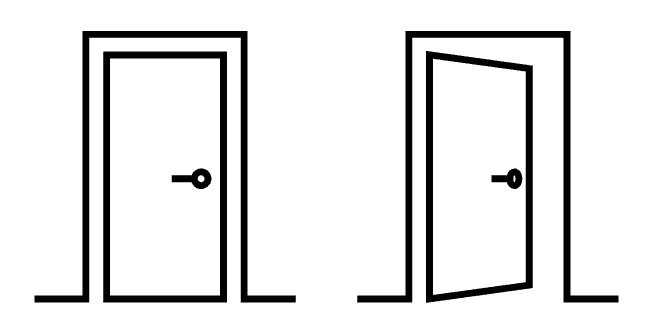
\includegraphics[width=0.5\linewidth]{porta}
	\end{figure}
	
	
\end{frame}

\begin{frame}{Item a scelta multipla forzata}
	
	\begin{quote}
		
		Preferisco un lavoro nel quale: 
		
		\begin{enumerate}
			\item Posso crescere come persona
			\item Posso guadagnare bene
			\item Posso imparare cose nuove
		\end{enumerate}
	\end{quote}
	
	
	\vspace{2.5mm}
	Le opzioni di risposta sono realmente ordinabili? Sono anche solo comparabili? Quale punteggio ottiene ogni alternativa?
	

	\begin{exampleblock}{Narcissistic Personality Inventory}
		\begin{enumerate}
			\item non sono né meglio né peggio di altre persone
			\item penso di essere una persona speciale 
		\end{enumerate}
		

		Una persona con un alto livello di narcisismo ha più probabilità di scegliere la seconda opzione
	\end{exampleblock}
\end{frame}

\begin{frame}{Rating scales}
	
	L'evoluzione delle scale con item Sì/No o Vero/Falso $\rightarrow$ aggiunta di livelli intermedi
	
	\emph{Summating rating scales:} Scale composte da diverse domande (\textbf{item}) il cui punteggio totale è ottenuto attraverso la somma dei punteggi alle valutazioni fornite ad ogni item
	
	\begin{block}{Assunzione}
		
		Il costrutto latente si muove lungo un continuum sottostante alle opzioni di risposte, ovvero è possibile dare una quantità alla variabile psicologica misurata a seconda dell'opzione di risposta scelta. 
	\end{block}
	
	
\end{frame}

\begin{frame}
	
	
	Esprimere il proprio livello di accordo con l'affermazione ``Sono una persona organizzata'' secondo le seguenti opzioni di risposta: 
	
	\begin{center}
		Per niente d'accordo:	$\square$ \hspace{2mm} $\square$ \hspace{2mm} $\square$ \hspace{2mm} $\square$ \hspace{2mm} $\square$: Completamente d'accordo
	\end{center}
	
	L'assunzione è che il livello di accordo con l'affermazione vari lungo un continuum e che questo continuum sia delimitato dagli ancoraggi ``Per niente d'accordo'' e ``Completamente d'accordo'': 
	
	\pause
	\begin{figure}
		\centering
		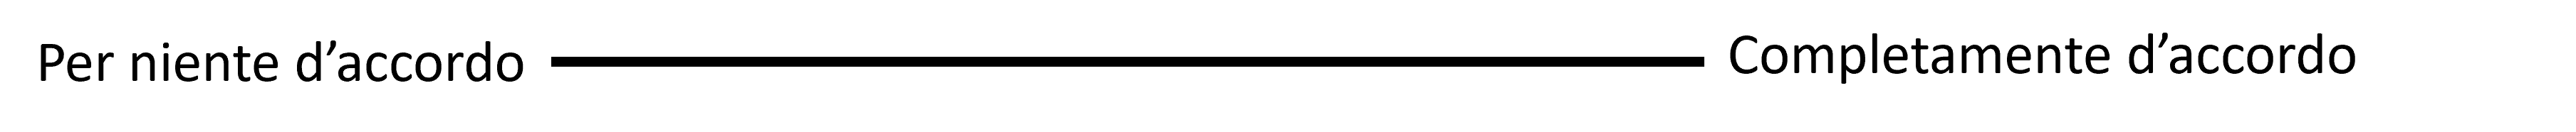
\includegraphics[width=0.9\linewidth]{accordo}
	\end{figure}
	
\end{frame}

\begin{frame}{``Sono una persona organizzata''}{Indicare il grado di accordo con l'affermazione}
	
	\begin{block}{Barrare il valore numerico corrispondente}
		
		\begin{tabular}{p{2cm} p{2cm}  p{2cm}  p{2cm}  p{2cm} }
			Per niente & & & & Completamente \\
			1 & 2 & 3 & 4& 5 \\
		\end{tabular}
	\end{block}
	
	\begin{block}{Barrare la casella}
		
		\begin{tabular}{p{2cm} p{2cm}  p{2cm}  p{2cm}  p{2cm} }
			Per niente & & & & Completamente \\
			$\square$ & $\square$ & $\square$ & $\square$& $\square$ \\
		\end{tabular}
	\end{block}
	
	\begin{block}{Segnare il numero}
		
		``Sono una persona organizzata'': \hspace{2cm} \large $\square$
	\end{block}
	
	
\end{frame}

\begin{frame}{Visual Analougue Scale}
	
	Molto utilizzate anche in psicologia dello sviluppo 
	
	\begin{figure}
		\centering
		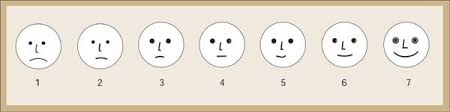
\includegraphics[width=0.7\linewidth]{vas}
	\end{figure}
	
\end{frame}

%\begin{frame}{Tipi di valutazione}
%	
%	\begin{block}{Accordo}
%		
%		Indicare il grado di accordo con un'affermazione
%		
%		Ad esempio:\\
%		\emph{Sono una persona organizzata} 
%		\begin{center}
%			Per niente d'accordo:	$\square$ \hspace{1.5mm} $\square$ \hspace{1.5mm} $\square$ \hspace{1.5mm} $\square$ \hspace{1.5mm} $\square$: Completamente d'accordo
%		\end{center}
%	\end{block}
%	
%	\begin{block}{Intensità}
%		
%		Dare una valutazione vera e propria rispetto a un argomento in termini di buono/cattivo, insufficiente/sufficiente, importante/non importante, eccetera. 
%		
%		Ad esempio: \\
%		\emph{Indicare il proprio livello di competenze informatiche}
%		\begin{center}
%			5 $=$ alto; \hspace{1.5mm} 4 $=$ medio-alto; \hspace{1.5mm} 3 $=$ medio; \hspace{1.5mm} 2 $=$ medio-basso; \hspace{1.5mm} 1 $=$ basso
%		\end{center}
%	\end{block}
%	
%	
%\end{frame}
%
%\begin{frame}
%	\begin{block}{Frequenza}
%		
%		Indicare la frequenza con cui vengono messi in atto i comportamenti o vengono sperimentati i vissuti descritti dall'item
%		
%		Ad esempio: \\
%		\emph{Nell'ultimo anno, mi sono sentito ansioso:}
%		\begin{center}
%			Mai	$\square$ \hspace{1.5mm} Raramente $\square$ \hspace{1.5mm} Qualche volta $\square$ \hspace{1.5mm} Spesso $\square$ \hspace{1.5mm} Sempre $\square$
%		\end{center}
%	\end{block}
%	
%	\pause
%	\begin{center}
%		Attenzione!
%	\end{center}
%	
%	Cosa vuole dire ``Spesso''? E ``Qualche volta''? Vogliono dire la stessa cosa per tutt*?
%\end{frame}

%\begin{frame}
%	
%	\begin{spacing}\Factor
%		\footnotesize
%		\begin{tabular}{|p{3.5cm}| c |c| c| c |c|}
%			\hline
%			Comportamento	&	Mai	&	Raramente	&	Qualche volta	&	Spesso	&	Sempre	\\\hline
%			\multicolumn{6}{|l|}{a}\\\hline
%			Leggere le mail	&		&		&		&		&		\\\hline
%			Scrollare Instagram	&		&		&		&		&		\\\hline
%			Guardare Netflix	&		&		&		&		&		\\\hline
%			\textbf{Andare al cinema}	&		&		&		&		&		\\\hline
%			\multicolumn{6}{|l|}{b}\\\hline
%			Prendere l'aereo	&		&		&		&		&		\\\hline
%			Comprare una lavatrice	&		&		&		&		&		\\\hline
%			Andare a sciare	&		&		&		&		&		\\\hline
%			\textbf{Andare al cinema}	&		&		&		&		&		\\\hline
%		\end{tabular}
%	\end{spacing}
%	
%	
%	
%\end{frame}
%
%\begin{frame}
%	
%	\begin{center}
%		Quante volte vai al cinema?
%	\end{center}
%	
%	
%	\vspace{1.5mm}
%	\pause
%	\begin{columns}[T]
%		\begin{column}{.50\linewidth}
%			\begin{center}
%				Bassa frequenza
%			\end{center}
%			\begin{enumerate}
%				\item Mai 
%				\item Circa una volta l'anno
%				\item Circa due volte l'anno
%				\item Due volte al mese 
%				\item Più di due volte al mese
%			\end{enumerate}
%		\end{column}
%		\pause
%		\begin{column}{.50\linewidth}
%			\begin{center}
%				Alta frequenza
%			\end{center}
%			\begin{enumerate}
%				\item Due volte al mese o meno 
%				\item Una volta a settimana
%				\item Due volte a settimana
%				\item Tutti i giorni 
%				\item Diverse volte al giorno
%			\end{enumerate}
%		\end{column}
%	\end{columns} 
%\end{frame}
%
%
%
%
%\begin{frame}{Quanti punti?}
%	Come regola generale, più è alto il numero di punti della scala, maggiore è poi l'attendibilità della misura
%	
%	Solitamente si considerano scale con un numero di punti tra 4 e 7 $\rightarrow$ Più di 7 punti sono ``Inutili''
%	
%	Numero dispari o numero pari di punti? 
%	
%	\pause
%	Un numero dispari di punti permette l'alternativa neutra: 
%	
%	\begin{itemize}
%		\item Ci sono dei casi (e.g., valutazione di soddisfazione per un servizio) dove ha senso avere un'alternativa neutra 
%		\item In altri casi (e.g., valutazione degli atteggiamenti verso un gruppo sociale) l'alternativa neutra funge da ``rifugio'' per non sbilanciarsi
%	\end{itemize}
%	
%	\begin{alertblock}{Attenzione!}
%		
%		La scala di risposta agli item e il numero di item somministrati vanno valutati insieme! \scriptsize Altrimenti è tortura 
%	\end{alertblock}
%\end{frame}
%
%\begin{frame}{Esempio I}
%	
%	Quanto sei soddisfatto dell'assistenza fornita da ciccio pasticcio gas \& energia?
%	
%	\begin{columns}[T]
%		\pause
%		\begin{column}{.50\linewidth}
%			\begin{enumerate}
%				\item Per nulla soddisfatto
%				\item Poco soddisfatto
%				\item Né soddisfatto né insoddisfatto
%				\item Abbastanza soddisfatto
%				\item Del tutto soddisfatto
%			\end{enumerate}
%		\end{column}
%		\pause
%		\begin{column}{.50\linewidth}
%			\begin{enumerate}
%				\item Per nulla soddisfatto
%				\item Poco soddisfatto
%				\item Abbastanza soddisfatto
%				\item Del tutto soddisfatto
%			\end{enumerate}
%		\end{column}
%	\end{columns}
%	
%\end{frame}
%
%\begin{frame}{Esempio II}
%	
%	Penso che gli immigrati debbano stare a casa loro		
%	
%	\begin{columns}[T]
%		\pause
%		\begin{column}{.50\linewidth}
%			\begin{enumerate}
%				\item Completamente in disaccordo
%				\item Un po' in disaccordo
%				\item Né d'accordo né in disaccordo
%				\item Un po' d'accordo
%				\item Completamente in accordo
%			\end{enumerate}
%		\end{column}
%		\pause
%		\begin{column}{.50\linewidth}
%			\begin{enumerate}
%				\item Completamente in disaccordo
%				\item Un po' in disaccordo
%				\item Un po' d'accordo
%				\item Completamente in accordo
%			\end{enumerate}
%		\end{column}
%	\end{columns}
%	
%\end{frame}

\begin{frame}{Criticità}
	\begin{block}{Acquiescienza}
		
		Essere sistematicamente d'accordo con le affermazioni proposte dagli item
	\end{block}
	
	\begin{block}{Estremismo}
		
		Scegliere sempre le risposte estreme
	\end{block}
	
	\begin{block}{Evasività}
		
		Scegliere sempre i punti centrali della scala o le risposte ``Non so''
	\end{block}
	
	\begin{block}{Desiderabilità sociale}
		
		Rispondere in modo da mostrarsi delle belle persone sempre e comunque	
	\end{block}
	
\end{frame}



\begin{frame}
	\begin{block}{Inaccuratezza}
		
		Rispondere a caso o in modo incoerente
	\end{block}
	
	
	\begin{block}{Devianza}
		
		Scegliere alternative di risposta volutamente insolite
	\end{block}
	
	\begin{block}{Produttività}
		
		Fornire ``troppe'' risposte o risposte troppo prolisse (in caso di domande aperte)
	\end{block}
	
	\begin{block}{Effetto alone}
		
		L'influenza della valutazione generale di sè quando si devono valutare degli aspetti specifici
	\end{block}
	
	\begin{block}{Indulgenza/Criticismo}
		
		Valutazioni sistematicamente sopra o sotto la media
	\end{block}
\end{frame}


\section[Misurazione implicita]{Misurazione implicita: Davvero la soluzione?}



\begin{frame}
	\vskip0pt plus 1fill
	Secondo Greenwald \& Banaji (1995), gli atteggiamenti impliciti sono definiti come:
	
	\vspace{5mm}
	\begin{quote}
		Introspectively unidentified -- or inaccurately identified -- traces of past experience that mediate favorable or unfavorable feelings, thoughts, or actions toward social objects
	\end{quote}
	
	\begin{center}
		\begin{large}
			IMPLICITO $=$ INCONSAPEVOLE
		\end{large}
	\end{center}
	
	Gli atteggiamenti impliciti si esprimono attraverso le cosiddette \textbf{associazioni automatiche}
	
	
	\vskip0pt plus 1filll
	
	\color{template}\rule{0.30\linewidth}{0.5pt}\\
	\color{black}
	\scriptsize{Greenwald, A. G., \& Banaji, M. R. (1995) Implicit Social Cognition: Attitudes, Self-Esteem, and Stereotypes.\emph{ Psychological Review}, 102-1, doi: 10.1037/0033-295X.102.1.4}
	
	
\end{frame}

\begin{frame}{Associazioni automatiche}
	\begin{center}
		
\includegraphics[width=.50\linewidth]{snakeFlower.png}
	\end{center}
	
	\begin{itemize}
		\item Non controllabili
		\item Attivate da stimoli ``triggering'' 
		\item Non accessibili attraverso l'introspezione 
		\item Veloci e quasi immediati
	\end{itemize}
	
	
\end{frame}

\begin{frame}{Associazioni automatiche e l'inconscio}
	Studiare le associazioni automatiche  $=$ Studiare gli atteggiamenti impliciti
	
	\vspace{3.5mm}
	\begin{center}
		
\includegraphics[width=.10\textheight]{down.png}
		
		\vspace{3.5mm}
		Avere accesso all'inconscio e poterlo (finalmente!) studiare con un approccio scientifico
	\end{center}
	
	\pause
	
	\centering
	
\includegraphics[width=.50\linewidth]{wrong.jpg}
	
\end{frame}

\begin{frame}
	\vskip0pt plus 1filll
	
	Fazio \& Olson (2003):
	
	\vspace{3mm}
	
	\begin{quote}
		Essere rapidi nell'associare i serpenti ad aggettivi o parole con valenza negativa non implica che non sia consapevoli dei propri atteggiamenti negativi verso i serpenti!
	\end{quote}
	
	\vspace{1.45mm}
	
	L'unica cosa di cui si è realmente inconsapevoli è che qualcuno sta misurando gli atteggiamenti!
	
	L'atteggiamento (l'oggetto della misura) non è implicito, lo è il processo stesso di misurazione
	
	
	\vspace{1.5mm}
	Costrutti misurati implicitamente Vs. Costrutti inconsapevoli 
	
	\vskip0pt plus 1filll
	
	\color{template}\rule{0.30\linewidth}{0.5pt}\\
	\color{black}
	\scriptsize{Fazio, R. H., \& Olson, M. A. (2003). Implicit measures in social cognition research: Their meaning
		and use. \emph{Annual Review of Psychology, 54}(1), 297–
		327. https://doi.org/10.1146/annurev.psych.54.101
		601.145225}
	
\end{frame}

\subsection*{Implicit $=$ indirect}


\begin{frame}
	
	\begin{center}
		Da
		
		\vspace{3.5mm}
		Esplicito = consapevole Vs. Implicito = inconsapevole/Inconscio  
		
		\emph{Riferendosi alla natura dei costrutti}
		\vspace{3.5mm}
		
		a:
		
		\vspace{3.5mm}
		Esplicito = diretto Vs. Implicito = indiretto 
		
		\emph{Riferendosi alla natura della misurazione}
	\end{center}
	
	\vspace{3.5mm}
	Significato \emph{empirico} del termine implicito
\end{frame}

\begin{frame}
	\vskip0pt plus 1filll
	Banaji \& Greenwald (2013): 
	
	\vspace{5mm}
	\begin{quote}
		Definizione \underline{\textbf{teorica}} del termine implicito come inconscio e inconsapevole
	\end{quote}
	
	\vspace{5mm}
	Greenwald \& Banaji (2017), Greenwald \& Lai (2020): 
	
	\vspace{5mm}
	\begin{quote}
		
		Definizione \underline{\textbf{empirica}} del termine implicito come indiretto 
		
	\end{quote}
	\vskip0pt plus 1filll
	
	\color{template}\rule{0.30\linewidth}{0.5pt}\\
	\color{black}
	\scriptsize{Banaji, M. R., \& Greenwald, A. G. (2013). \emph{Blindspot:
			Hidden biases of good people}. Delacorte Press,\\ 
		Greenwald, A. G., \& Banaji, M. R. (2017). The
		implicit revolution: Reconceiving the relation
		between conscious and unconscious. \emph{American Psychologist, 72}(9), 861–871. https://doi.org/10.1037/
		amp0000238\\
		Greenwald, A. G., \& Lai, C. K. (2020). Implicit social
		cognition. \emph{Annual Review of Psychology, 71}, 419–
		445. https://doi.org/10.1146/annurev-psych-010419-
		050837
	}
\end{frame}

\begin{frame}{Perché...?}
	\begin{itemize}
		\item Mancanza di evidenza empirica scientifica per poter sostenere l'accesso all'inconscio 
		\item Problemi relativi alla validità di costrutto $\rightarrow$ cosa stiamo misurando? Siamo \emph{sicuri} di star misurando quello che pensiamo di misurare?  
		\item Definizione senza una teoria dietro 
	\end{itemize}
\end{frame}

\section[Associazioni automatiche]{Misure implicite basate sulle associazioni automatiche}

\subsection{Implicit Association Test}

%\begin{frame}
%	\begin{center}
%		\url{https://www.millisecond.com/download/library}
%	\end{center}
%	
%	\begin{figure}
%		\centering
%		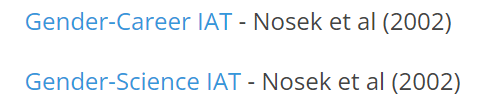
\includegraphics[width=\linewidth]{milli}
%	\end{figure}
%	
%\end{frame}


\begin{frame}
	
	\tikzoverlay (n1) at (8cm, 0.5cm){%
		\begin{minipage}{0.3\linewidth}
			\centering	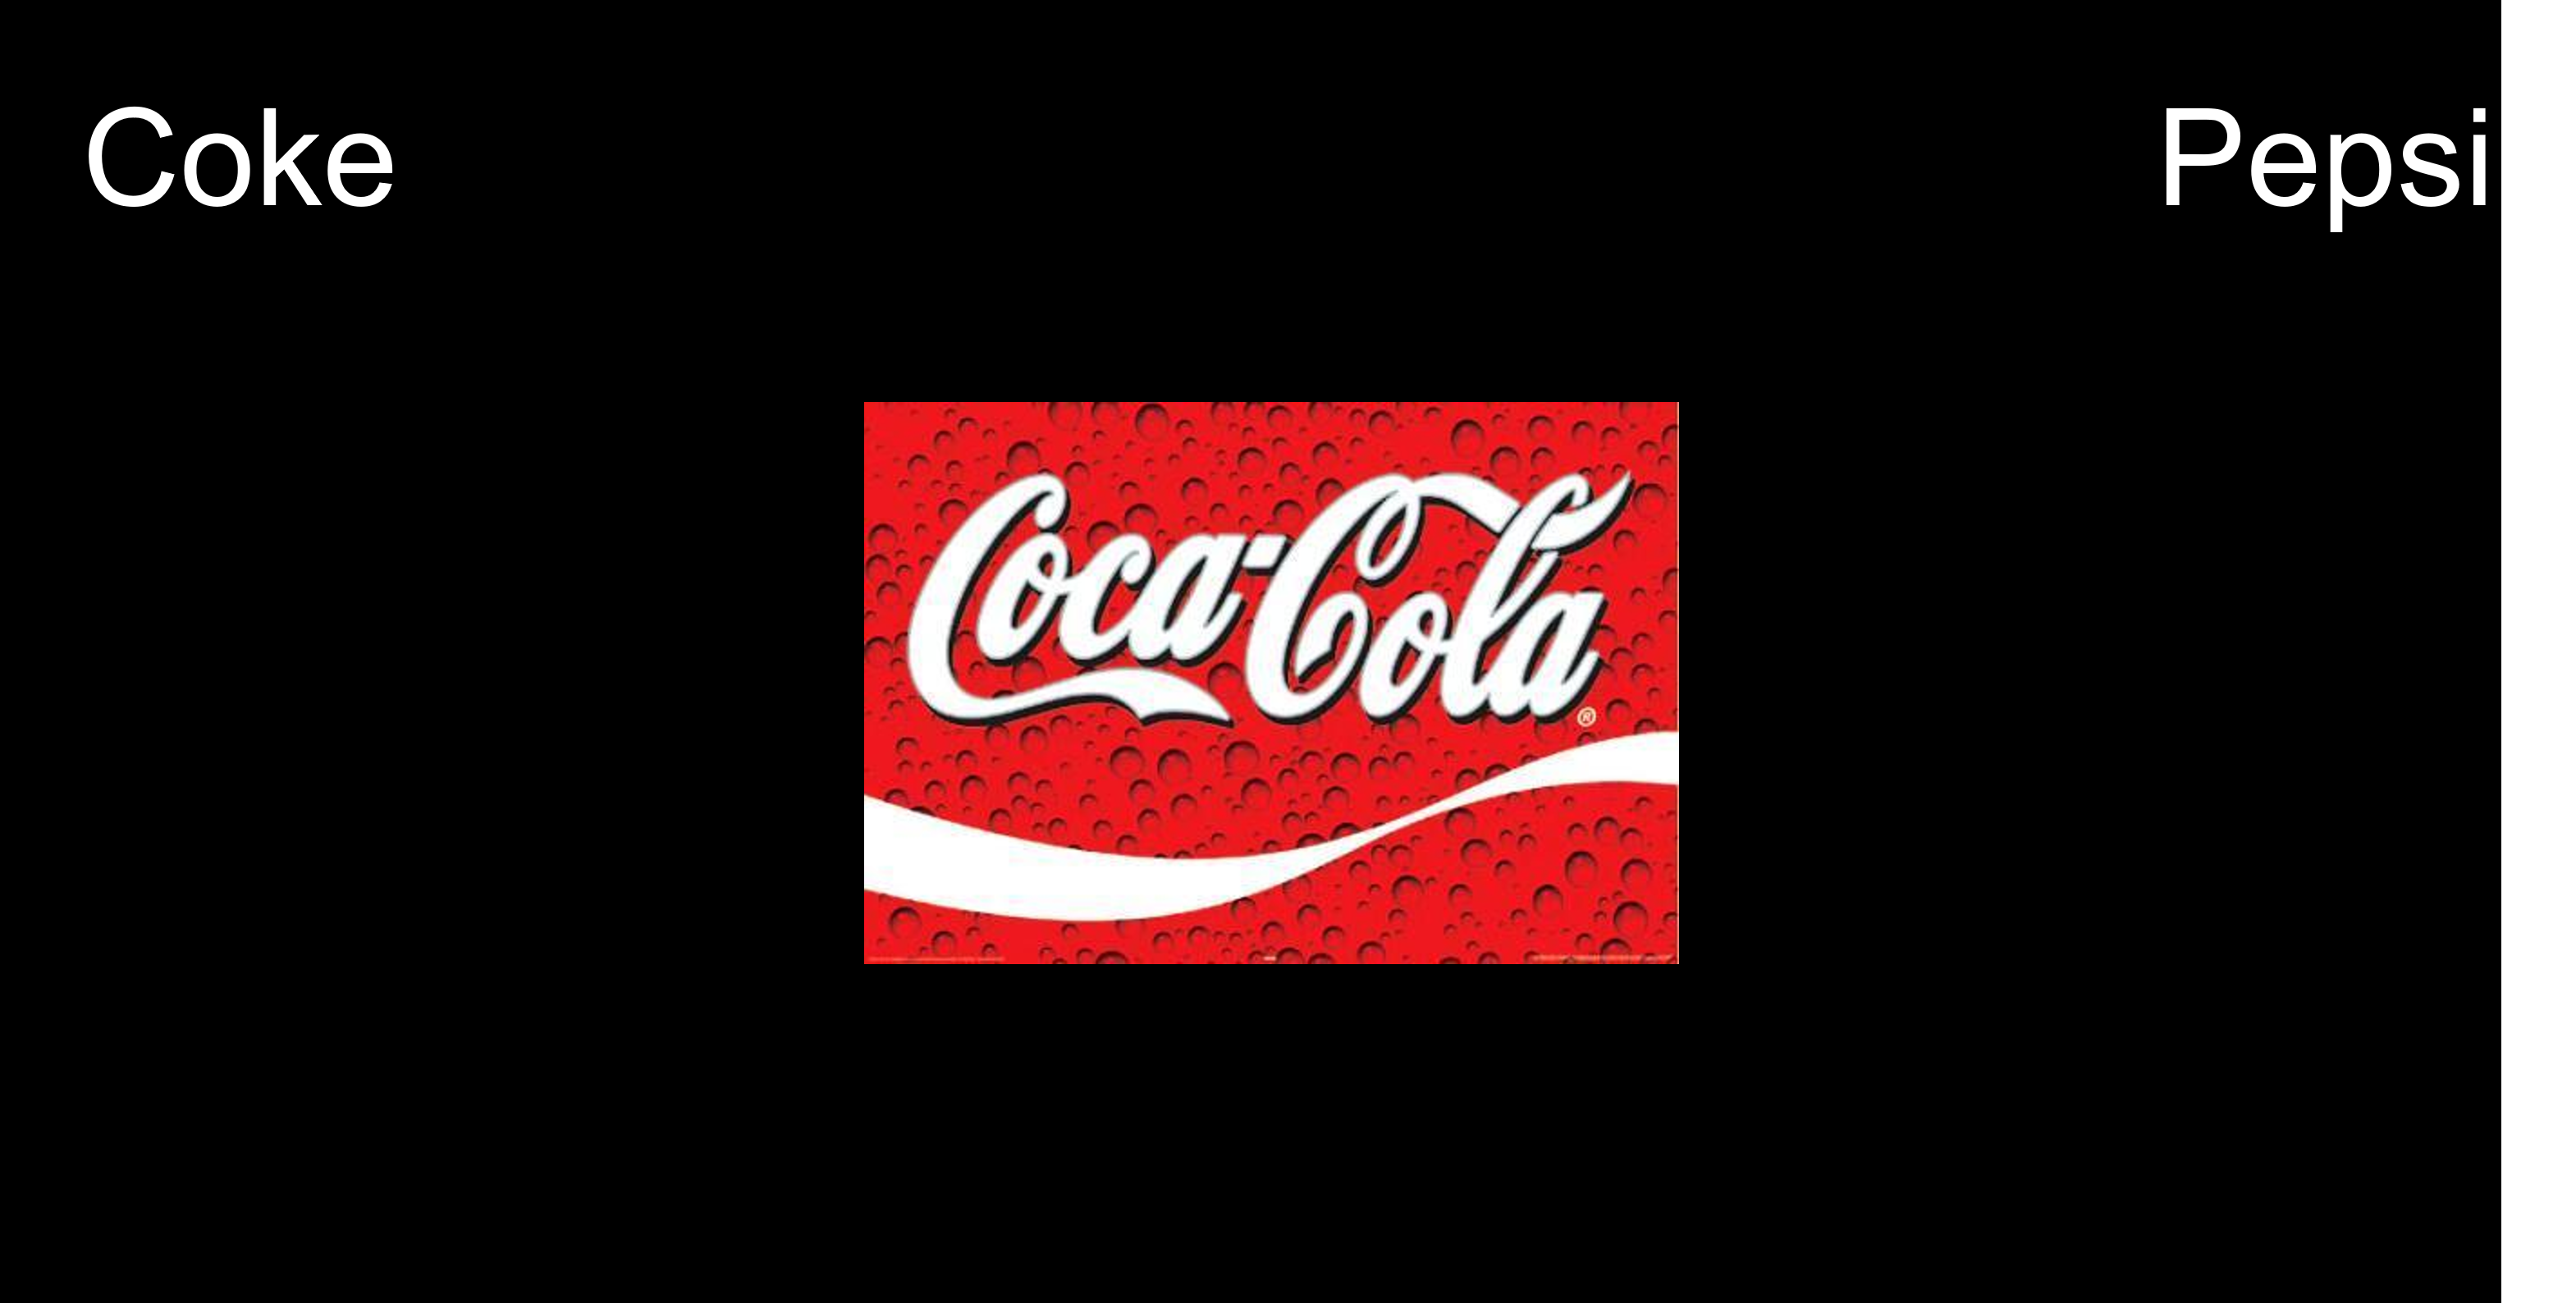
\includegraphics[width=\linewidth]{iatbase.png}
		\end{minipage}
	}; %
	
	
	\begin{table}
		\centering
		\caption{IAT}
		\begin{tabular}{c c c c }
			\hline
			Blocco	&	\# Trial	&	Tasto sinistro (E)	&	Tasto destro (I)	\\ \hline
			1	&	20	&	Good	&	Bad	\\
			2	&	20	&	Coke	&	Pepsi	\\
			\textcolor<2->{unipd}{3}	&	\textcolor<2->{unipd}{20}	&	\textcolor<2->{unipd}{Coke + Good}	&	\textcolor<2->{unipd}{Pepsi + Bad}	\\
			\textcolor<2->{unipd}{4}	&	\textcolor<2->{unipd}{40}	&	\textcolor<2->{unipd}{Coke + Good}	&	\textcolor<2->{unipd}{Pepsi + Bad}	\\
			5	&	20	&	Pepsi	&	Coke	\\
			\textcolor<3->{blu}{6}	&	\textcolor<3->{blu}{20}	&	\textcolor<3->{blu}{Pepsi + Good}	&	\textcolor<3->{blu}{Coke + Bad}	\\
			\textcolor<3->{blu}{7}	&	\textcolor<3->{blu}{40}	&	\textcolor<3->{blu}{Pepsi + Good}	&	\textcolor<3->{blu}{Coke + Bad}	\\
			\hline
		\end{tabular}
	\end{table}
	
	
	
	
	\vspace{2mm}
	\begin{columns}
		\begin{column}{.50\linewidth}
			\onslide<2-> \textcolor{unipd}{Condizione Coke-Good/Pepsi-Bad}	
		\end{column}
		\begin{column}{.50\linewidth}
			\onslide<3-> \textcolor{blu}{Condizione Pepsi-Bad/Coke-Good}	
		\end{column}
		
	\end{columns}
	
In caso di errore $\rightarrow$ X rossa sullo schermo che blocca la compilazione
\end{frame}


\begin{frame}
	\begin{columns}
		\column{.5\linewidth}
		\centering{\textcolor{unipd}{Coke-Good/Pepsi-Bad (CGPB)}}
		\begin{figure}
			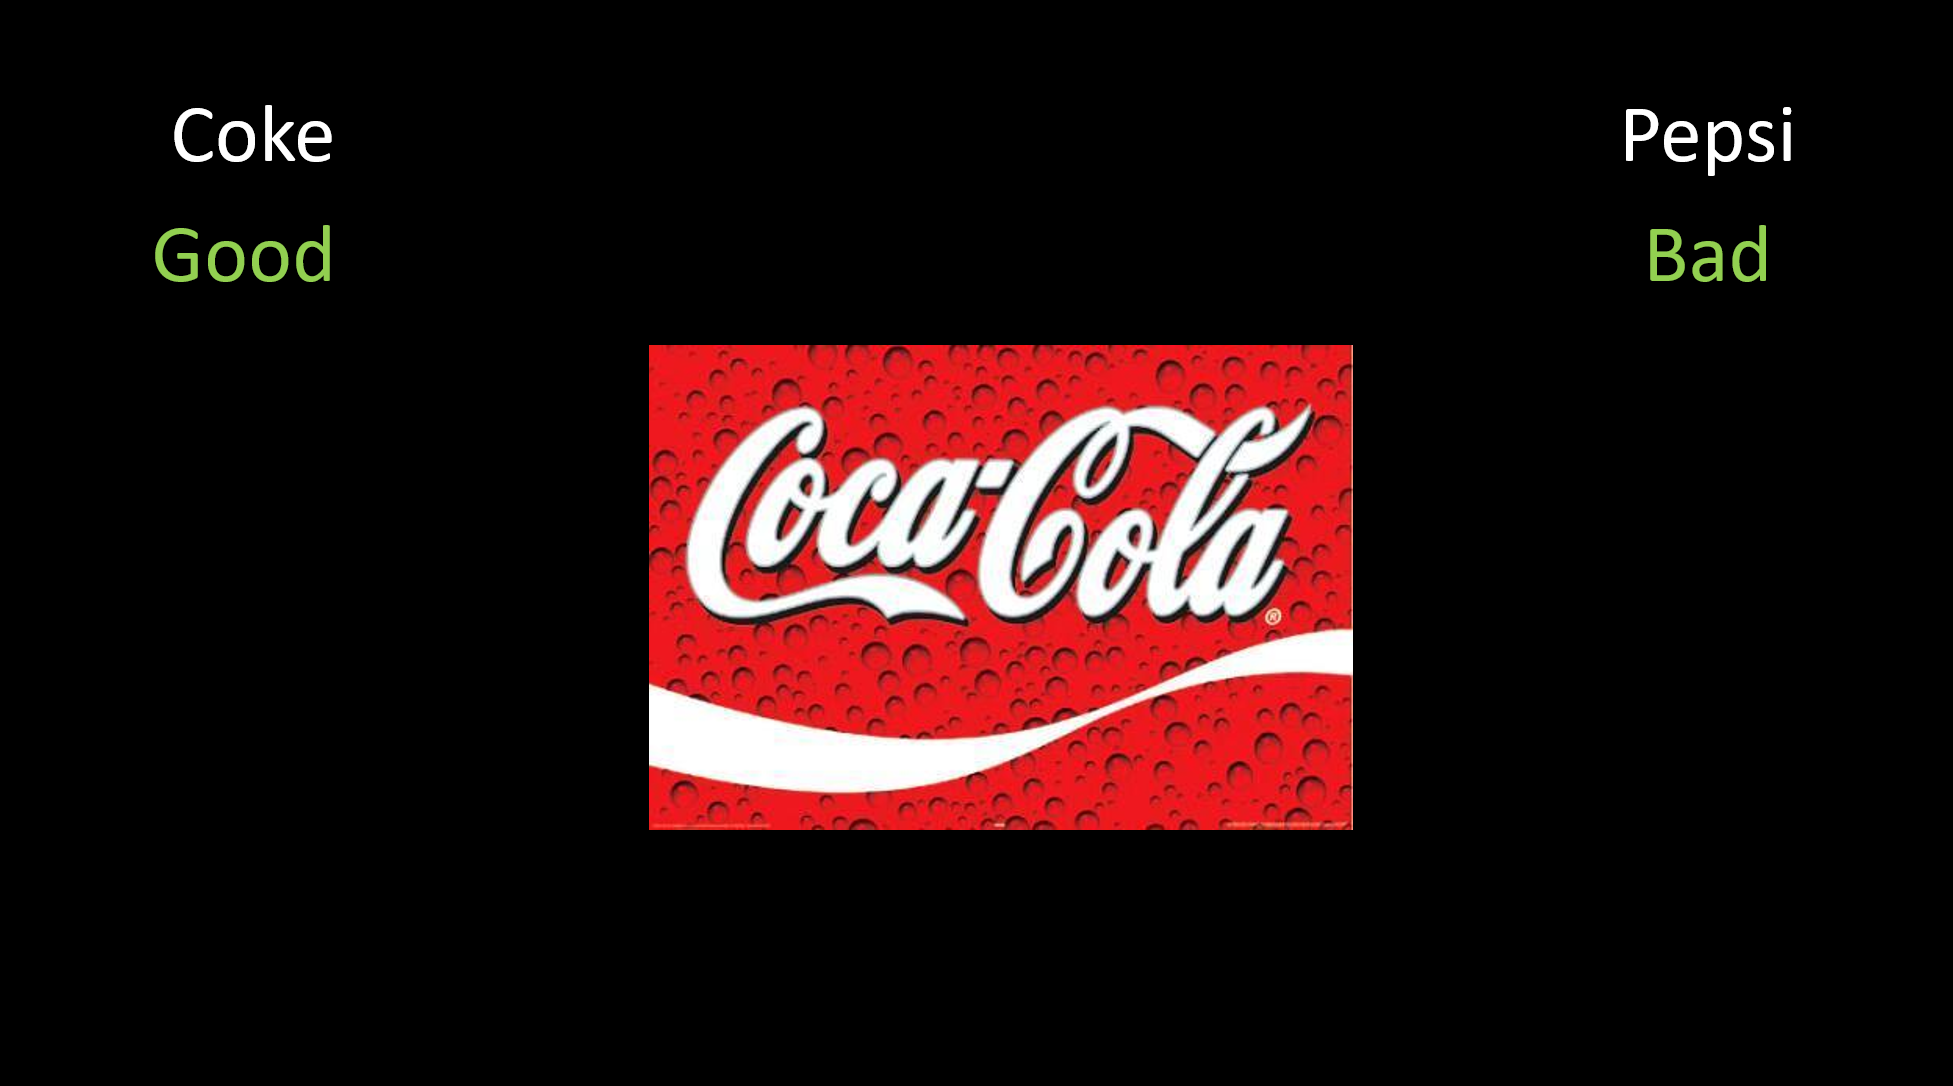
\includegraphics[width=\linewidth]{cocagood.png}
		\end{figure}
		
		\column{.5\linewidth}
		\centering{\textcolor{blu}{Pepsi-Good/Coke-Bad (PGCB)}}
		\begin{figure}
			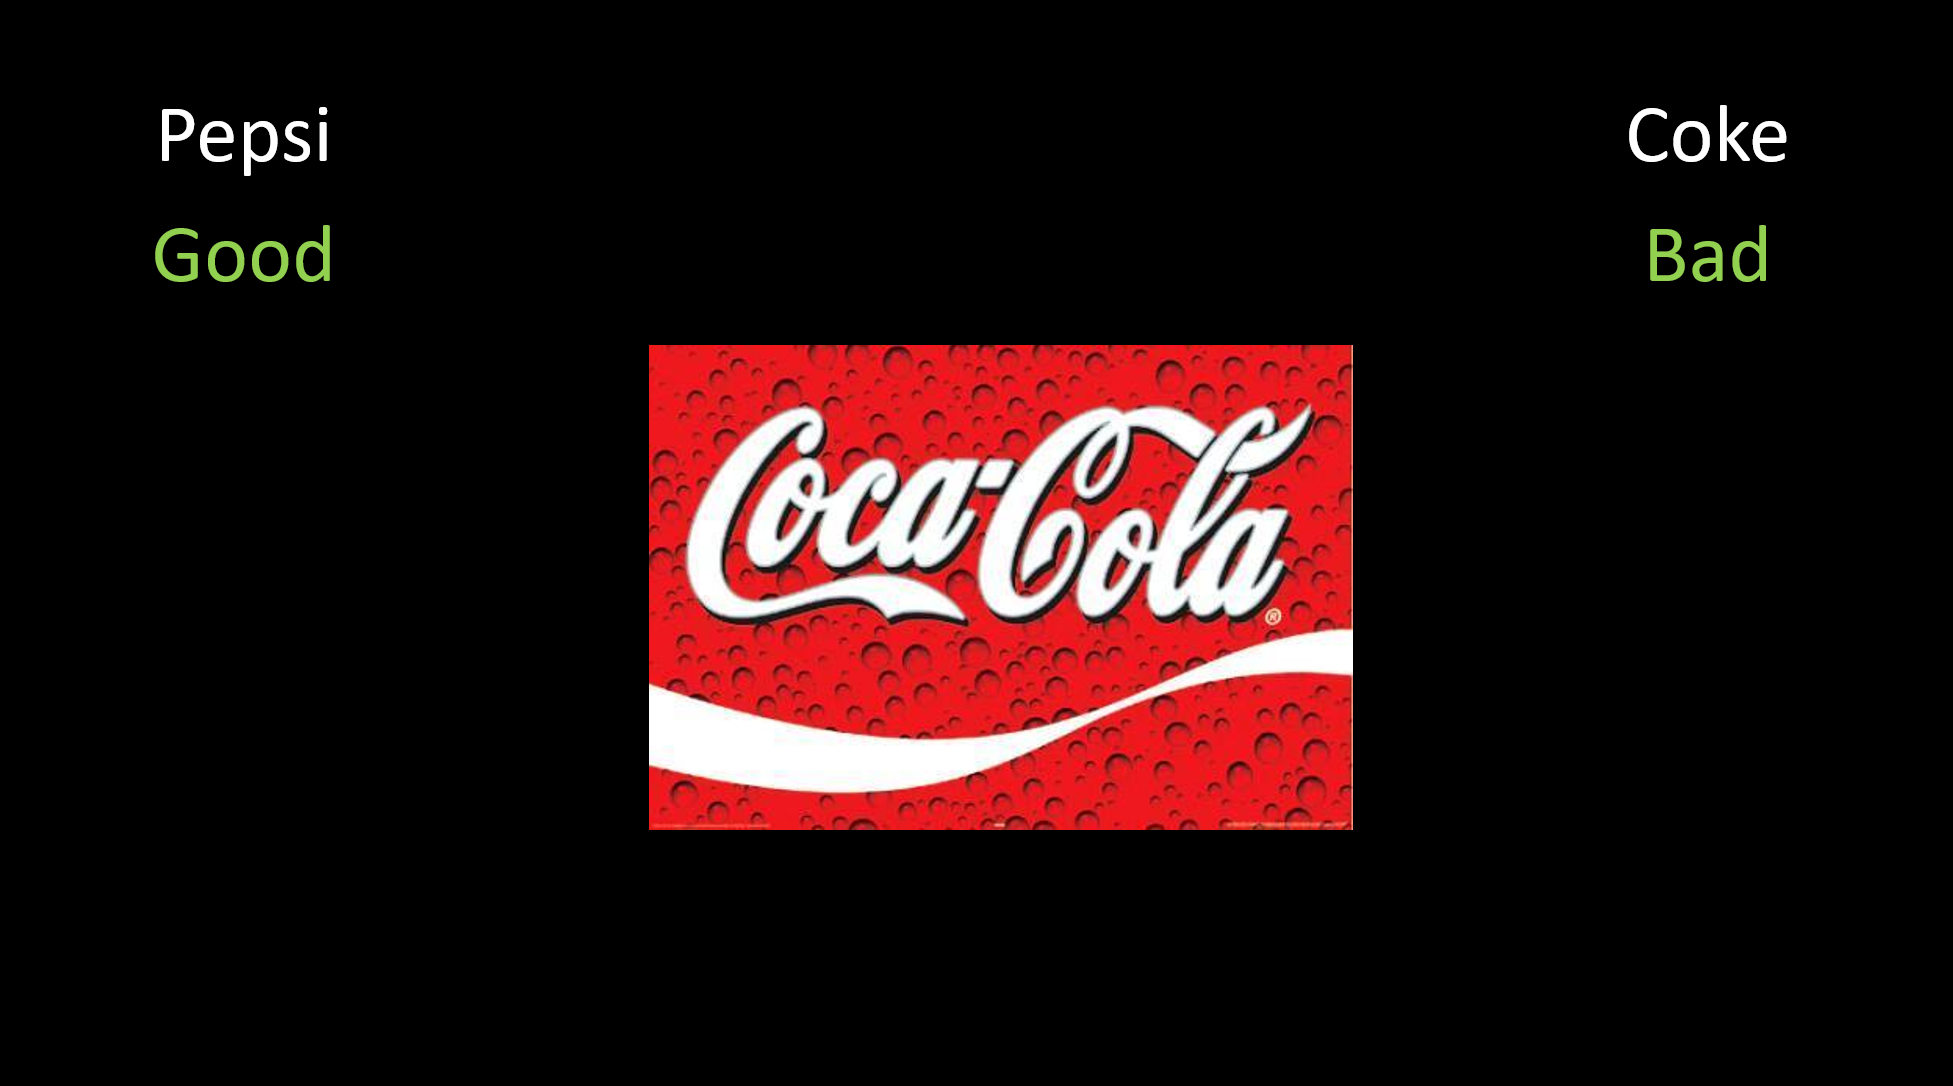
\includegraphics[width=\linewidth]{cocabad.png}
		\end{figure}
	\end{columns}
	
\end{frame}

\begin{frame}
	\begin{columns}
		\column{.5\linewidth}
		\centering{\textcolor{unipd}{Coke-Good/Pepsi-Bad (CGPB)}}
		\begin{figure}
			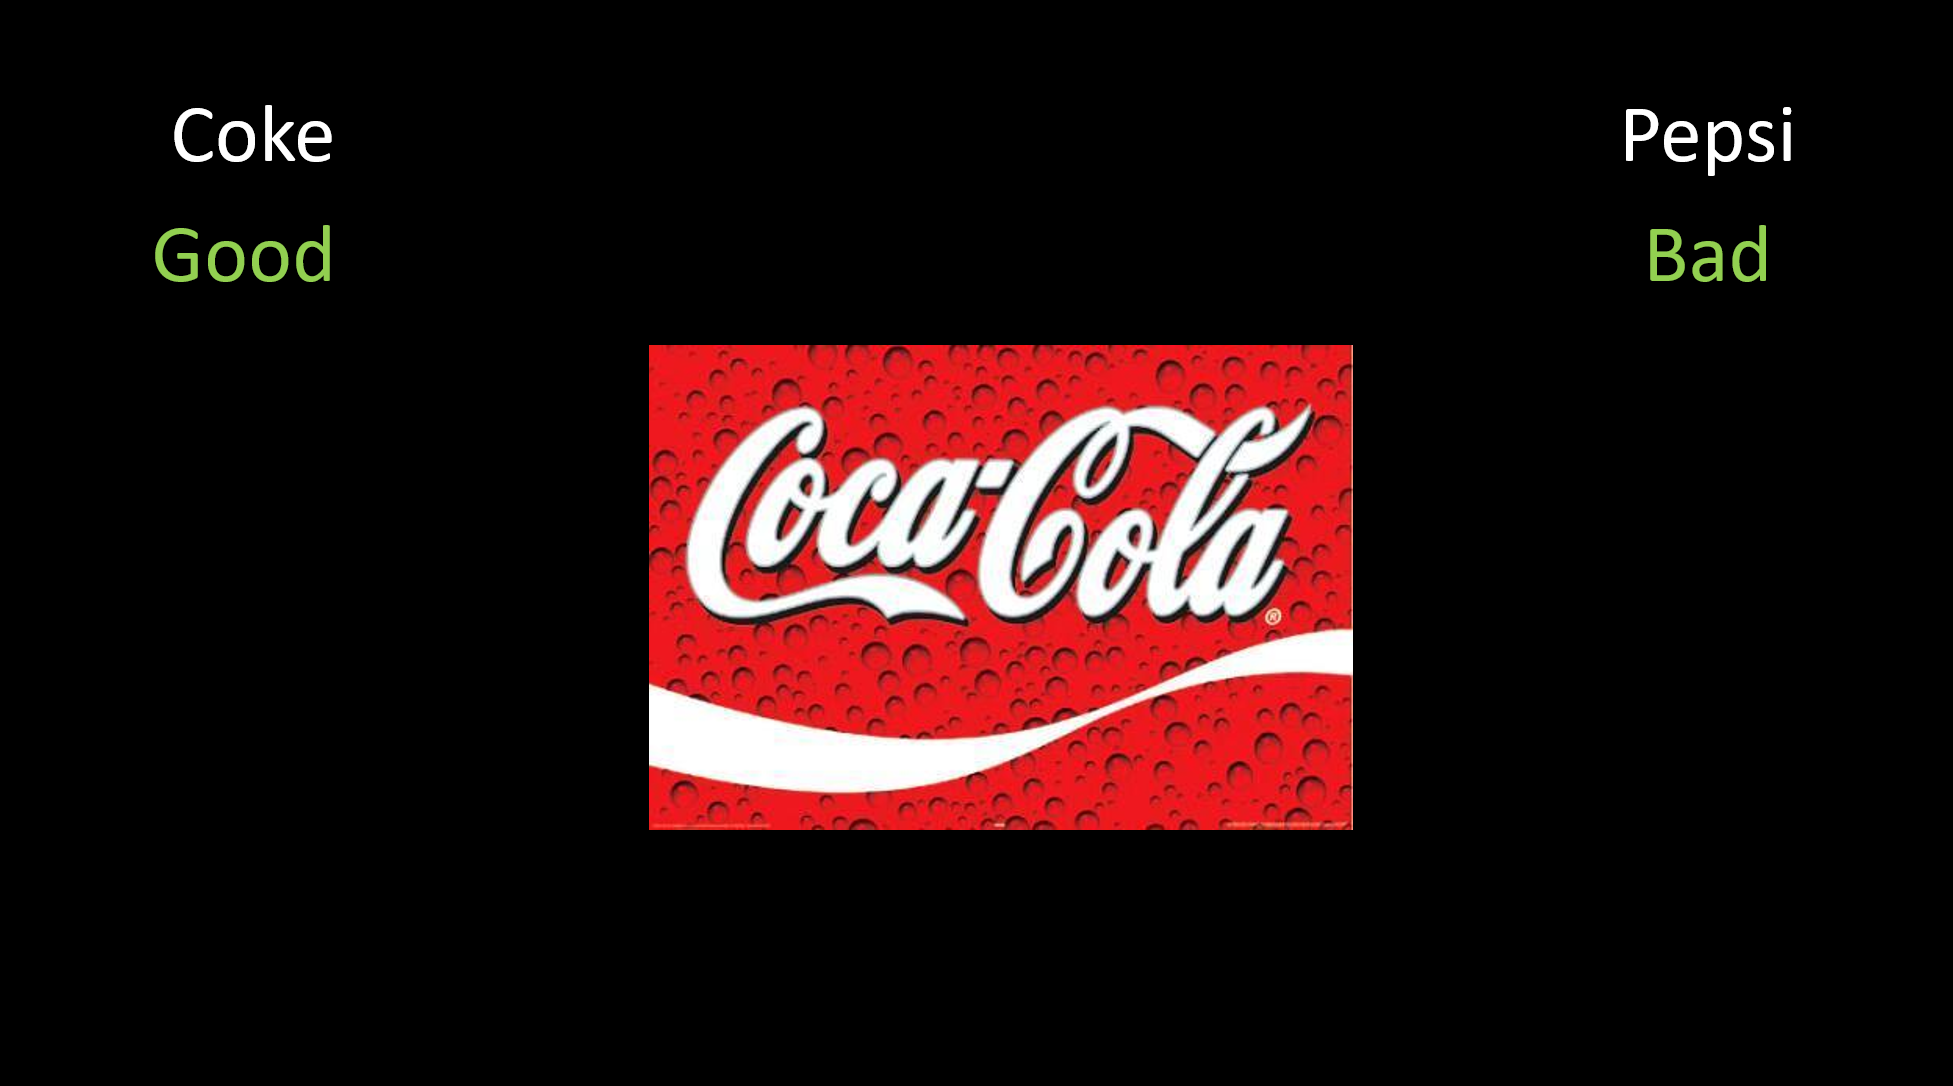
\includegraphics[width=\linewidth]{cocagood.png}
		\end{figure}
		
		\column{.5\linewidth}
		\centering{\textcolor{blu}{Pepsi-Good/Coke-Bad (PGCB)}}
		\begin{figure}
			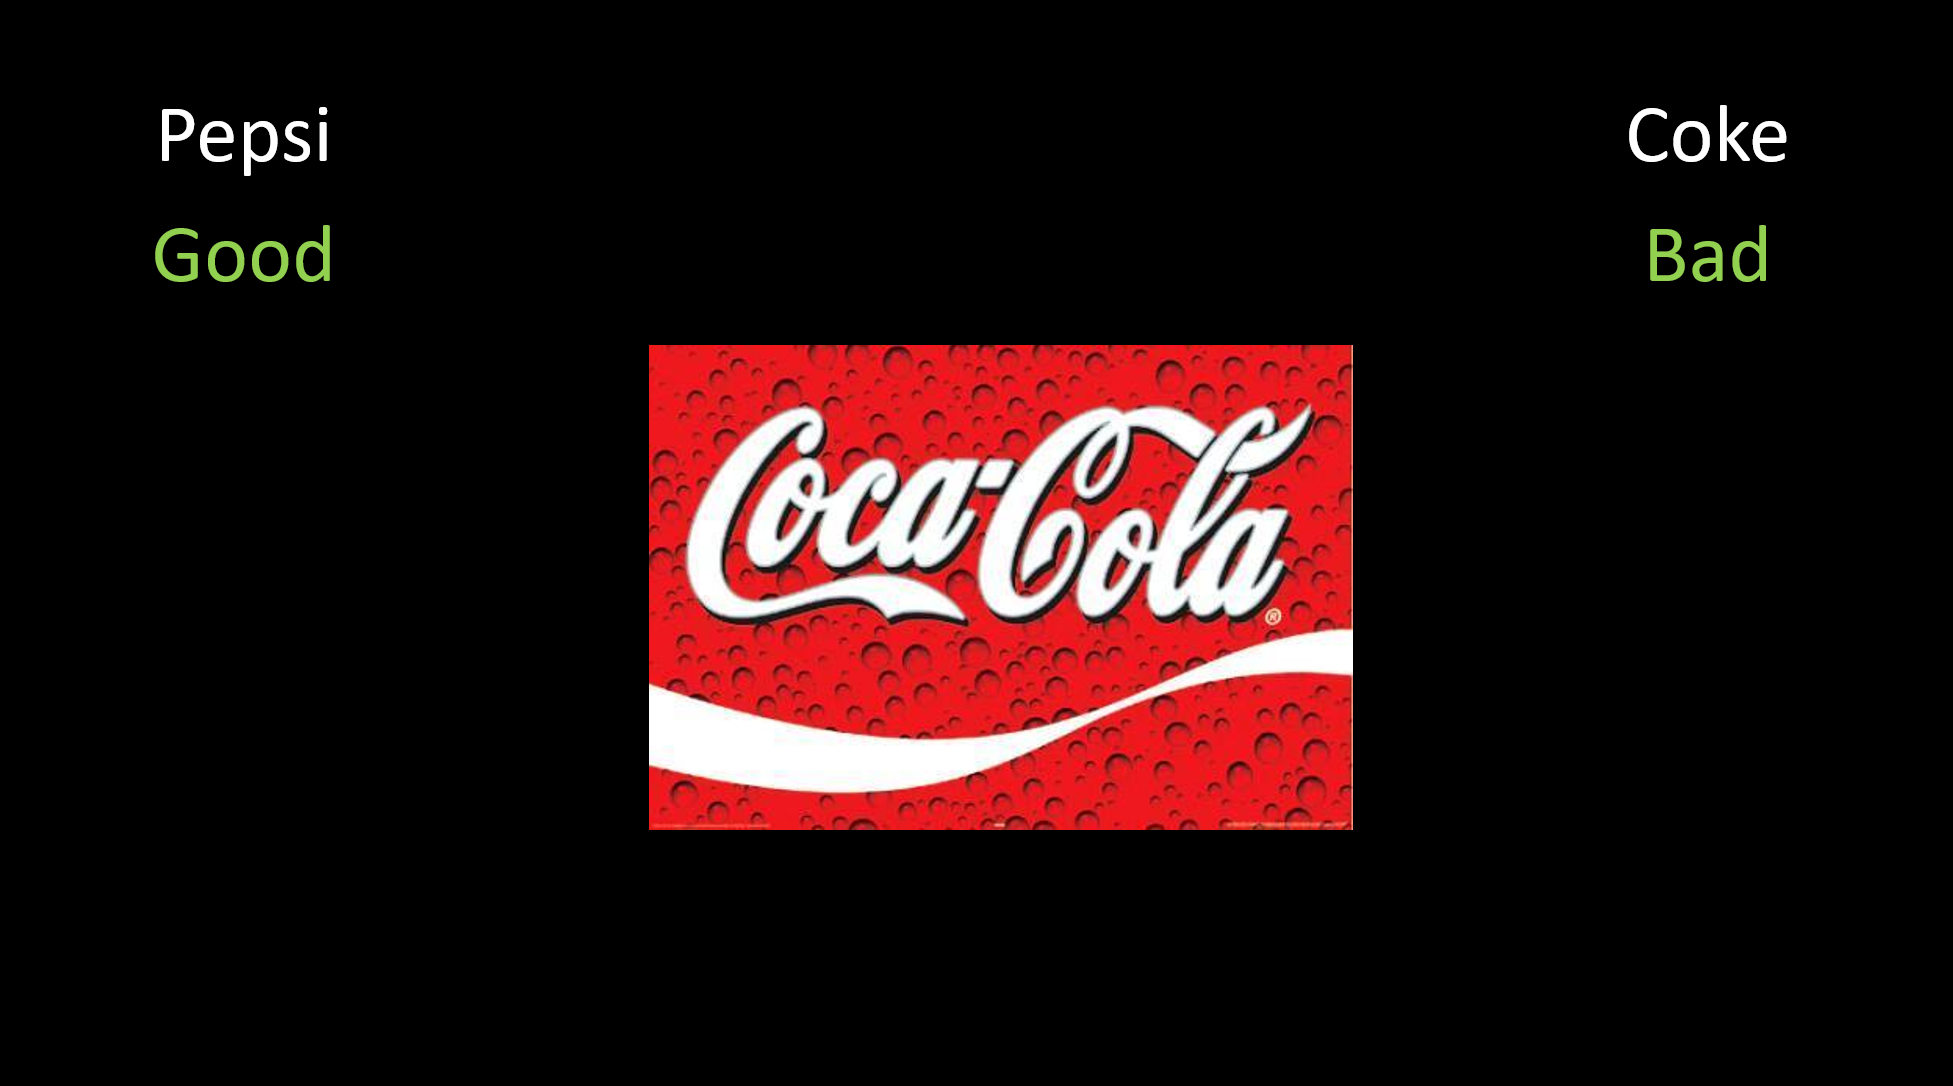
\includegraphics[width=\linewidth]{cocabad.png}
		\end{figure}
	\end{columns}
	
\end{frame}


\begin{frame}
	\begin{textblock*}{10cm}(0.5cm,1cm)
		{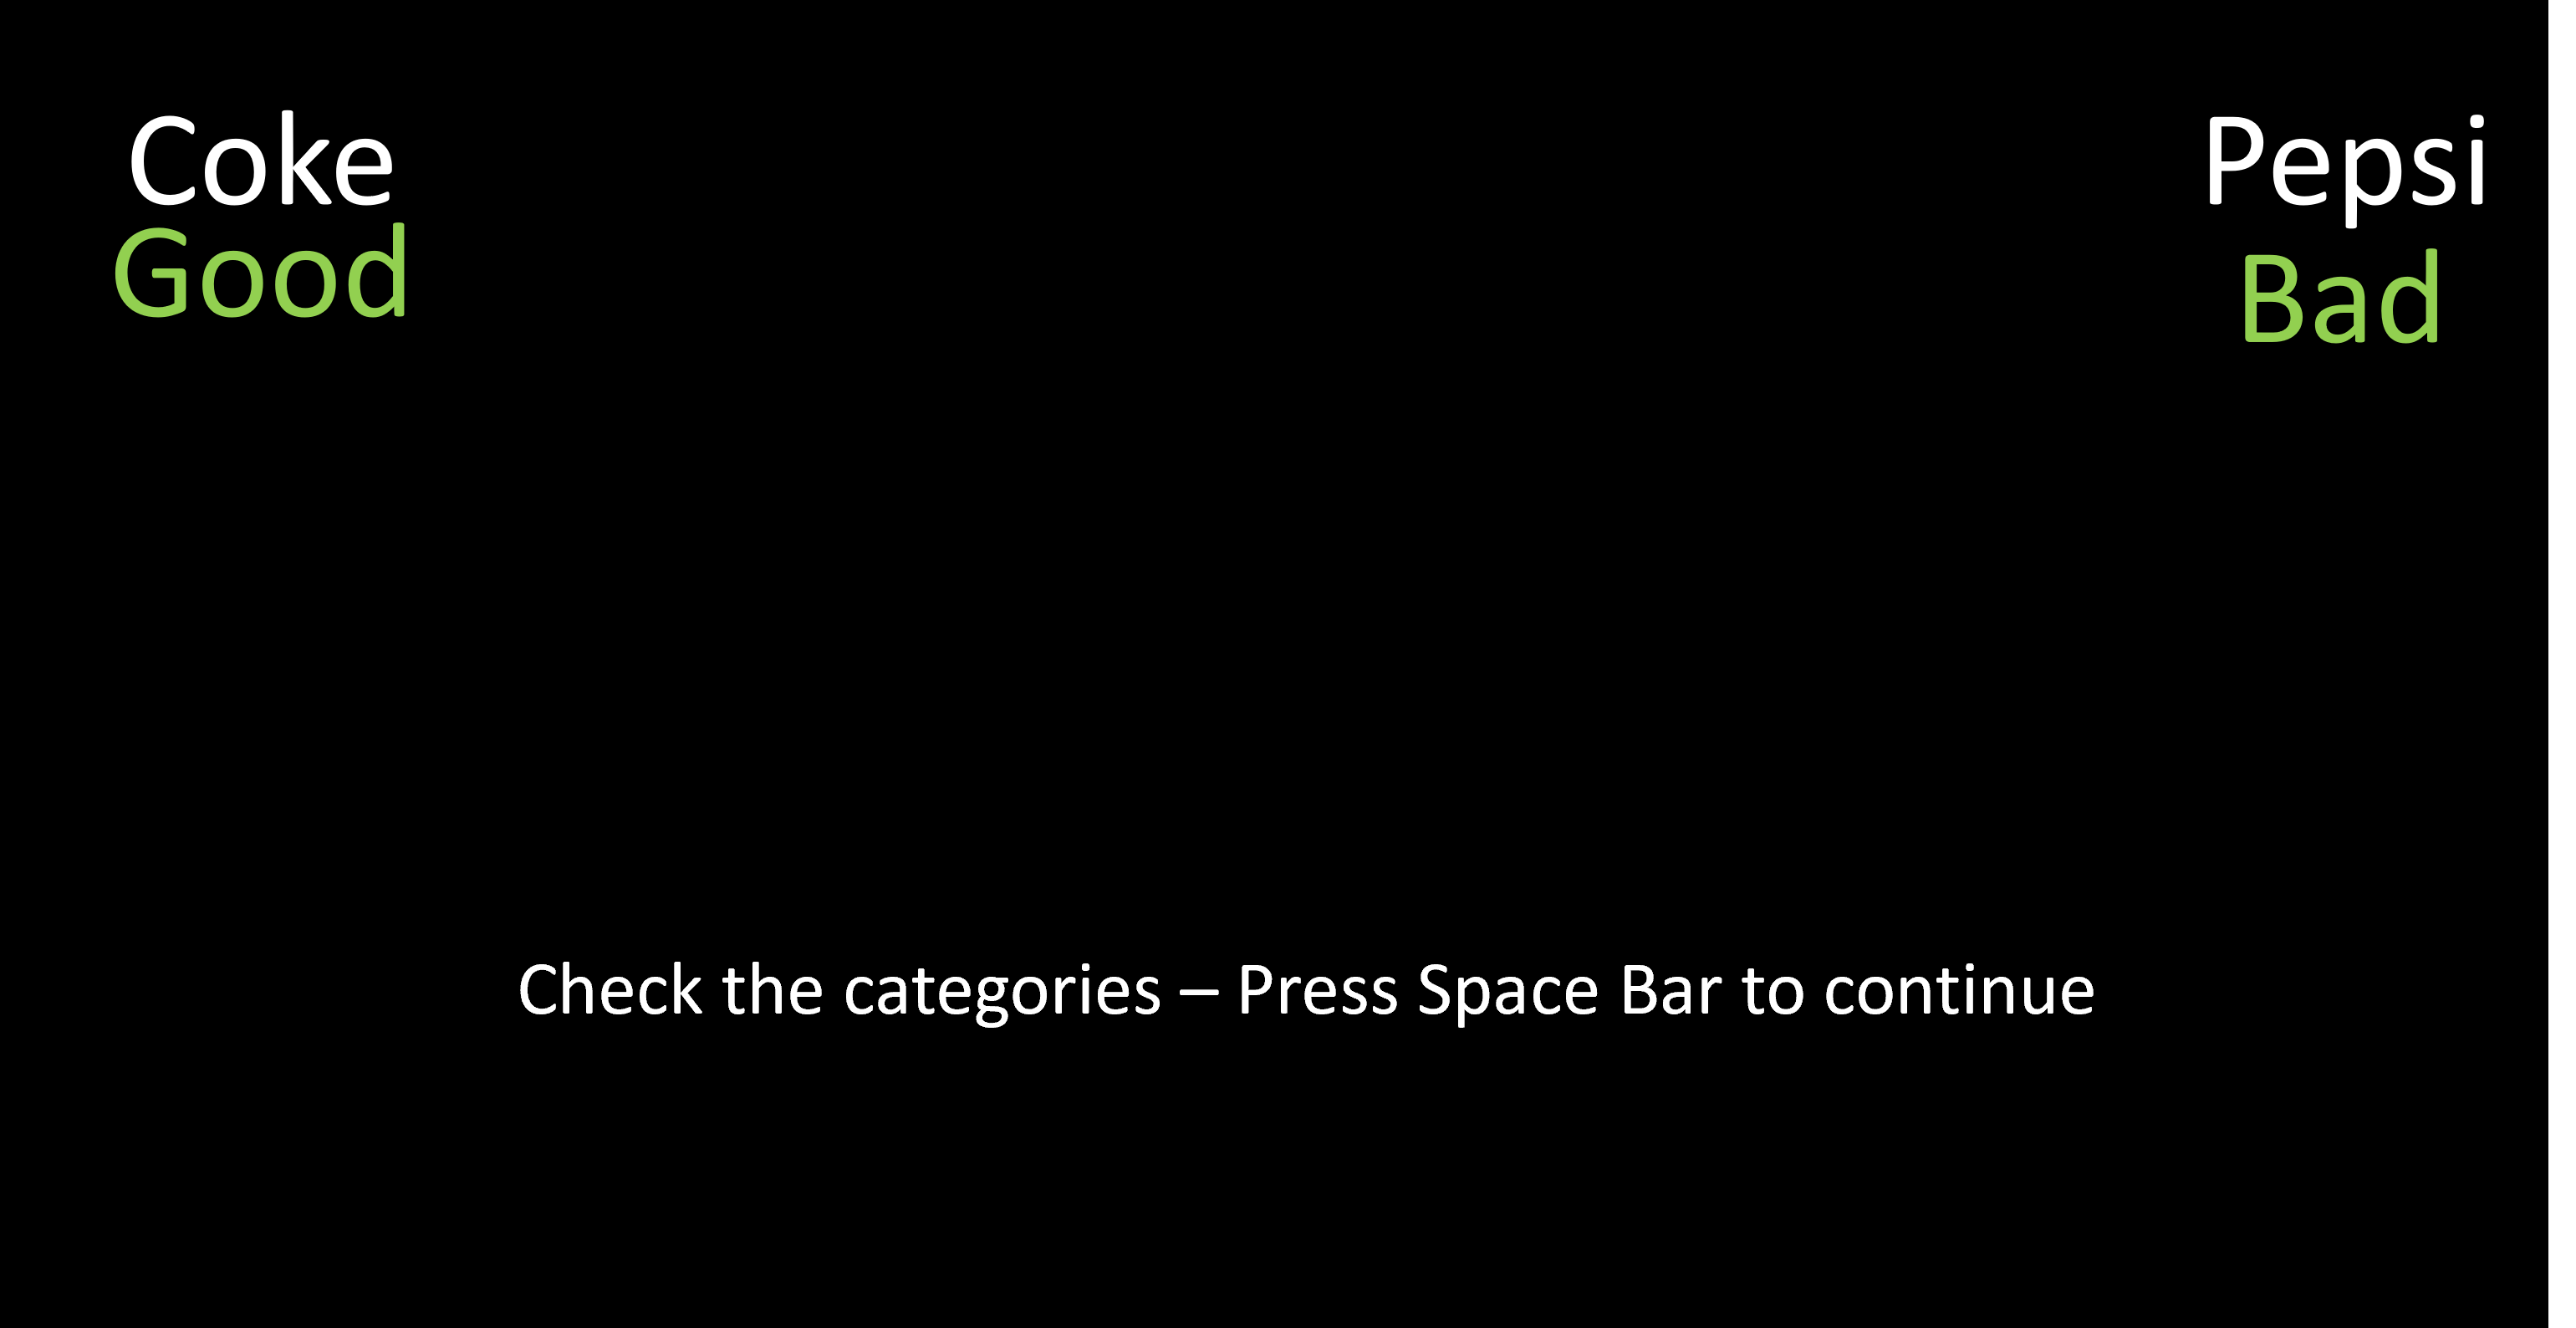
\includegraphics[width=\linewidth]{cokeIAT1.png}}
	\end{textblock*}
	\begin{textblock*}{10cm}(0.7cm,1.4cm)
		{\includegraphics<2->[width=\linewidth]{cokeIAT2.png}}
	\end{textblock*}
	\begin{textblock*}{10cm}(0.9cm,1.8cm)
		{\includegraphics<3->[width=\linewidth]{cokeIAT3.png}}
	\end{textblock*}
	\begin{textblock*}{10cm}(1.1cm,2.2cm)
		{\includegraphics<4->[width=\linewidth]{cokeIAT4.png}}
	\end{textblock*}
	\begin{textblock*}{10cm}(1.3cm,2.6cm)
		{\includegraphics<5->[width=\linewidth]{cokeIAT5.png}}
	\end{textblock*}
	
	\vskip0pt plus 1filll
	
	\onslide<2-2> Tasto E
	\onslide<3-3> Tasto I
	\onslide<4-4> Tasto E
	\onslide<5-5> Tasto I
	
\end{frame}

\subsection*{Scoring}

\begin{frame}{\emph{D} score}
	\vskip0pt plus 1filll
	Greenwald et al. (2003)
	
	\vspace{5mm}
	\begin{columns}
		\begin{column}{.50\linewidth}
			$$D_{\mathrm{B6,B3}} = \frac{M_{\mathrm{B6}} - M_{\mathrm{B3}}}{sd_{\mathrm{B6, B3}}}$$
		\end{column}
		\begin{column}{.50\linewidth}
			$$D_{\mathrm{B7,B4}} = \frac{M_{\mathrm{B7}} - M_{\mathrm{B4}}}{sd_{\mathrm{B7, B4}}}$$
		\end{column}
	\end{columns}
	
	\vspace{5mm}
	\begin{equation*}
		D = \frac{D_{\mathrm{B6,B3}} + D_{\mathrm{B7,B4}}}{2}
	\end{equation*}
	
	\pause
	\vspace{5mm}
	Risposte errate? Risposte troppo veloci?
	
	\vskip0pt plus 1filll
	
	\color{template}\rule{0.30\linewidth}{0.5pt}\\
	\color{black}
	\scriptsize{Greenwald, A. G., Nosek, B. A., \& Banaji, M. R.
		(2003). Understanding and using the implicit association test: I. An improved scoring algorithm. \emph{Journal
			of Personality and Social Psychology, 85}(2), 197–
		216. https://doi.org/10.1037/0022-3514.85.2.197}
\end{frame}

\begin{frame}
	
	\begin{spacing}\Factor
		\begin{table}[th!]
			\centering
			\caption{\label{tab:overview} Panoramica degli algoritmi di scoring}
			\scalebox{.9}{
						\begin{tabular}{llll}
				\hline
				\emph{D score} & Risposte errate & Risposte troppo veloci\\\hline
				\emph{D1} & Built-in correction & No \\
				\emph{D2} & Built-in correction & Eliminare trials $<$ 400 \emph{ms} \\
				\emph{D3} & Mean (correct responses) + 2\emph{sd} & No\\
				\emph{D4} & Mean (correct responses) + 600 \emph{ms} & No \\
				\emph{D5} & Mean (correct responses) + 2\emph{sd} & Eliminare trials $<$ 400 \emph{ms}\\
				\emph{D6} & Mean (correct responses) + 600 \emph{ms} & Eliminare trials $<$ 400 \emph{ms} \\\hline
			\end{tabular}
			}

		\end{table}
	\end{spacing}
\end{frame}


\begin{frame}
	\begin{figure}
		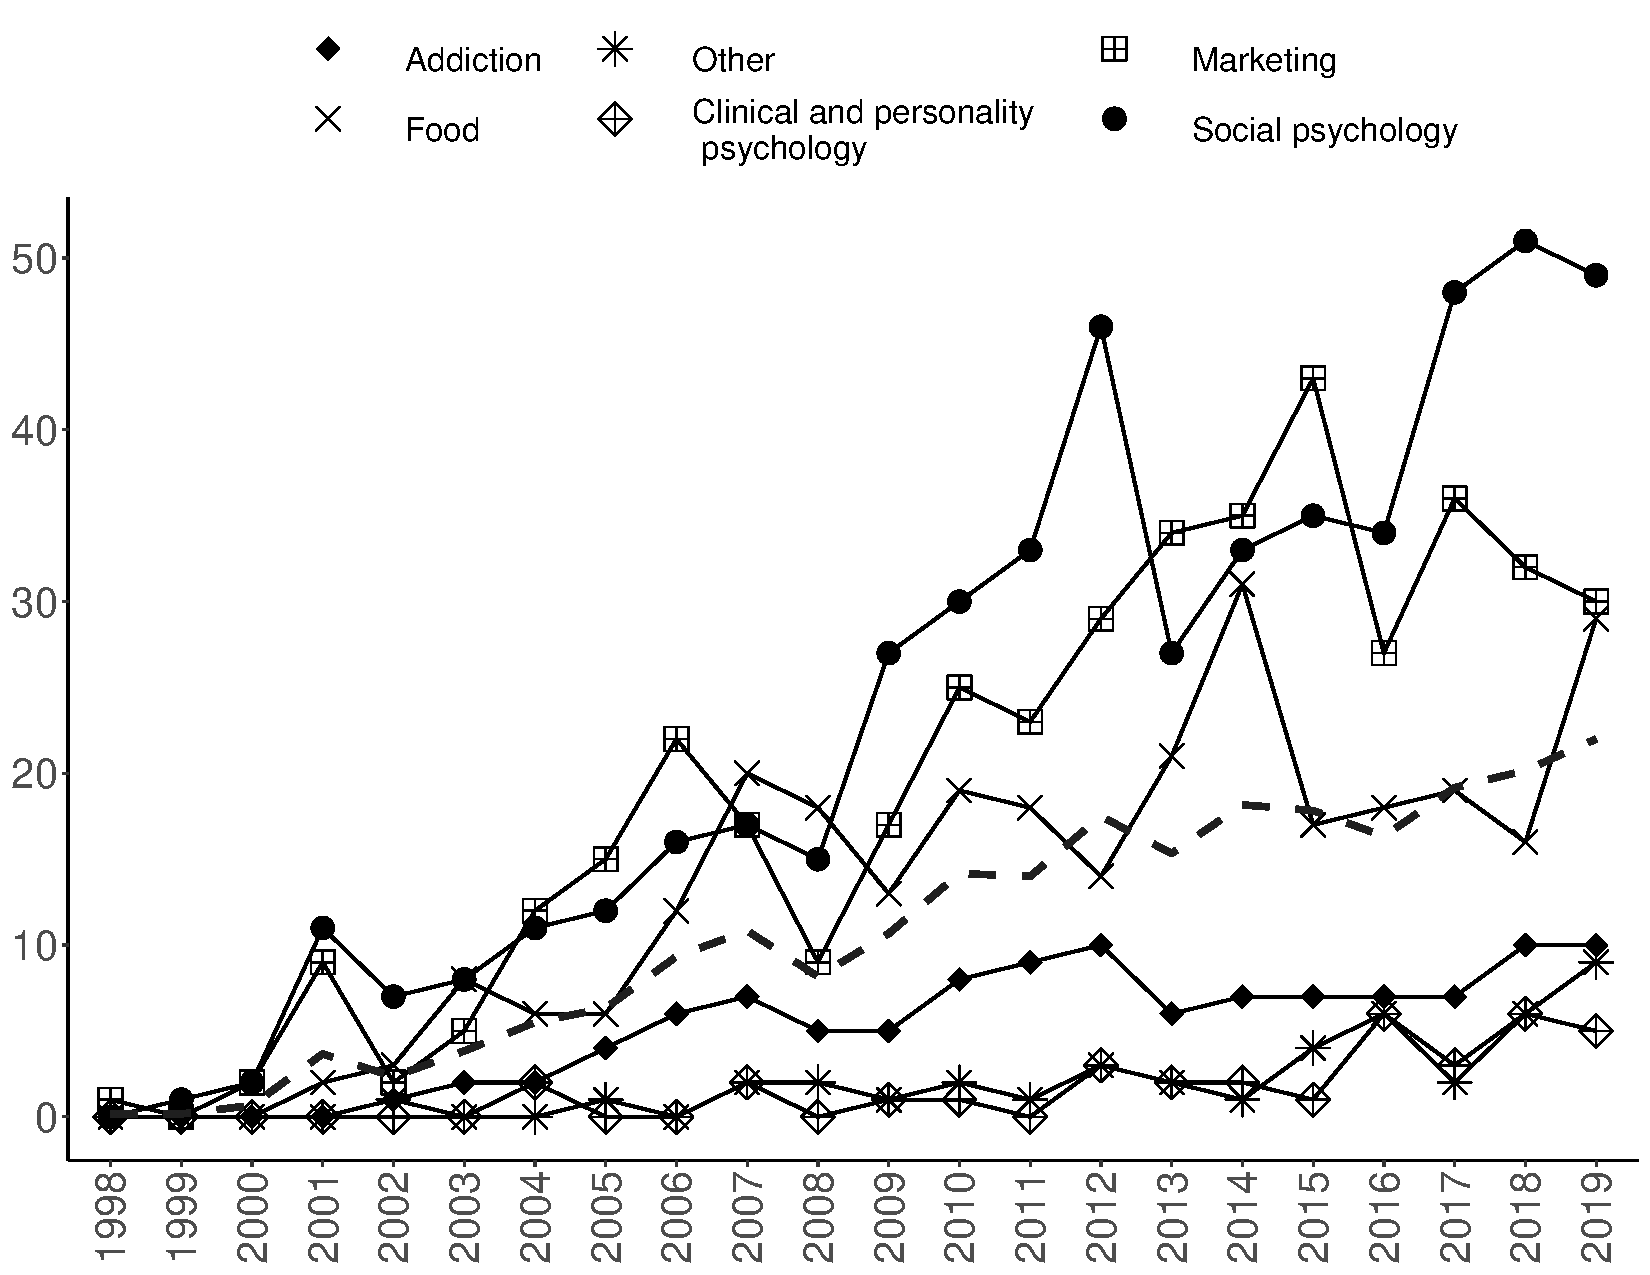
\includegraphics[width=.80\linewidth]{yearsIAT.pdf}
	\end{figure}
\end{frame}


\begin{frame}{Uno dei problemi dello IAT}
	\onslide<1->
	\tikzoverlay (n1) at (1cm, 1cm){%
		\begin{minipage}{0.1\linewidth}
			\centering	
\includegraphics[width=\linewidth]{coca3.jpg}
		\end{minipage}
	}; %
	\onslide<1->
	\tikzoverlay (n2) at (7cm, 1cm){%
		\begin{minipage}{0.4\linewidth}
			\centering	
\includegraphics[width=0.25\linewidth]{pepsi3.jpg}
		\end{minipage}
	}; %
	\onslide<1->
	\tikzoverlay (n3) at (5cm, 0.5cm){%
		\begin{minipage}{0.4\linewidth}
			\huge \textbf{vs}
		\end{minipage}
	}; %	
	
	\onslide<2->
	
	\vspace{10mm}
	IAT $\rightarrow$ Misura \emph{comparativa} di quanto piace un oggetto rispetto al suo ``opposto''
	
	\vspace{5mm}
	\pause
	Problemi: 
	\begin{itemize}
		\item Non è sempre facile trovare un oggetto che sia effettivamente l'opposto rispetto all'oggetto di interesse 
		\vspace{2.5mm}
		\item La misura che si ottiene dell'oggetto di interesse in realtà dipende dalla categoria di contrasto che si è deciso di utilizzare! 
		\vspace{2.5mm}
		\item Ci sono casi in cui è più utile ottenere una misura ``assoluta'' rispetto a un oggetto di interesse 
	\end{itemize}
	
\end{frame}

\begin{frame}{Single Category IAT}
	
	\onslide<1->
	\tikzoverlay (n1) at (10cm, 1cm){%
		\begin{minipage}{0.1\linewidth}
			\centering	
\includegraphics[width=\linewidth]{coca3.jpg}
		\end{minipage}
	}; %
	
	
	Karpinski \& Steinman (2006):
	
	\begin{spacing}\Factor
		\begin{table}
			\centering
			\caption{SC-IAT}
			\begin{tabular}{c c c c}
				\hline
				Blocco	&	\# Trial	&	Tasto sinistro (E)	&	Tasto destro (I)	\\
				\hline
				1	&	24	&	Good + Coke	&	Bad	\\
				\textcolor<2->{unipd}{2}	&	\textcolor<2->{unipd}{72}	&	\textcolor<2->{unipd}{Good + Coke}	&	\textcolor<2->{unipd}{Bad}	\\
				3	&	24	&	Good 	&	Bad + Coke	\\
				\textcolor<3->{blu}{4}	&	\textcolor<3->{blu}{72}	&	\textcolor<3->{blu}{Good}	&	\textcolor<3->{blu}{Bad + Coke}	\\
				\hline
			\end{tabular}
		\end{table}
	\end{spacing}
	
	\begin{columns}
		\begin{column}{.50\linewidth}
			\centering
			\onslide<2->
			\textcolor{unipd}{Coke-Good condition}
		\end{column}
		
		\begin{column}{.50\linewidth}
			\onslide<3->
			\centering
			\textcolor{blu}{Coke-Bad condition}
		\end{column}
	\end{columns}
	
	\vspace{5mm}
	\onslide<4->
	\begin{itemize}
		\item Response Time Window (rtw, solitamente a 1,500 ms)
		\item Feedback ad ogni risposta data
	\end{itemize}
	
	
\end{frame}

\begin{frame}
	\begin{columns}
		\column{.5\linewidth}
		\centering{\textcolor{unipd}{Coke-Good}}
		\begin{figure}
			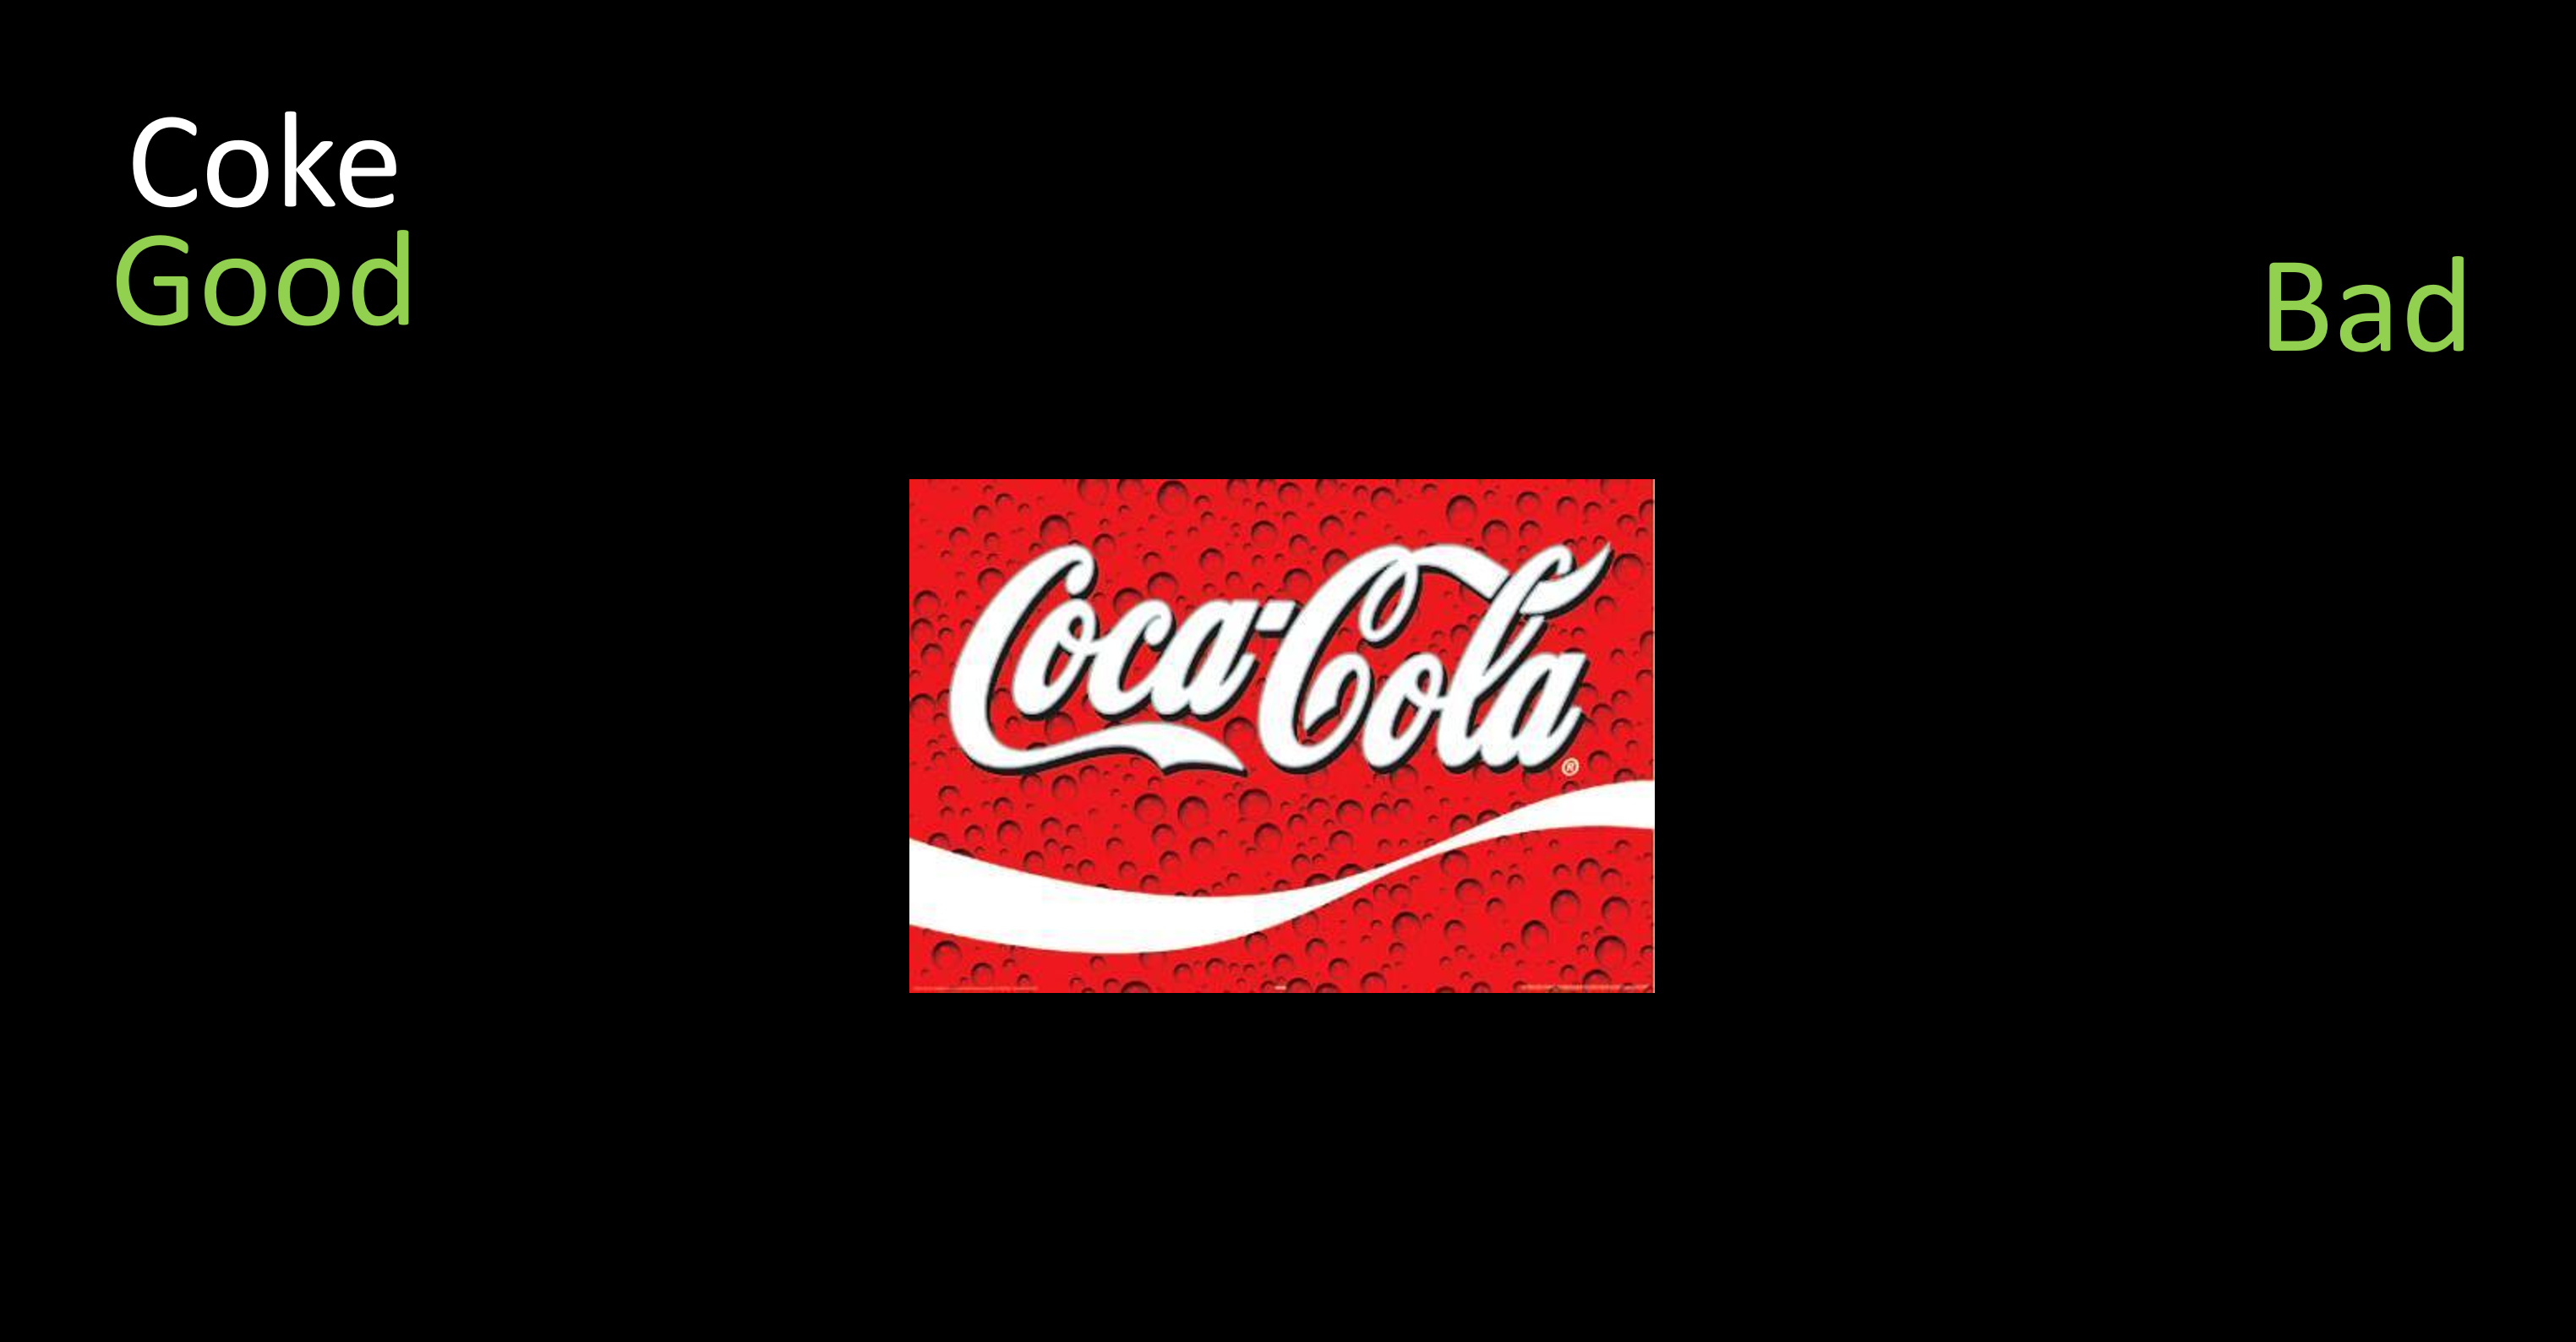
\includegraphics[width=\linewidth]{scGood.png}
		\end{figure}
		
		\column{.5\linewidth}
		\centering{\textcolor{blu}{Coke-Bad}}
		\begin{figure}
			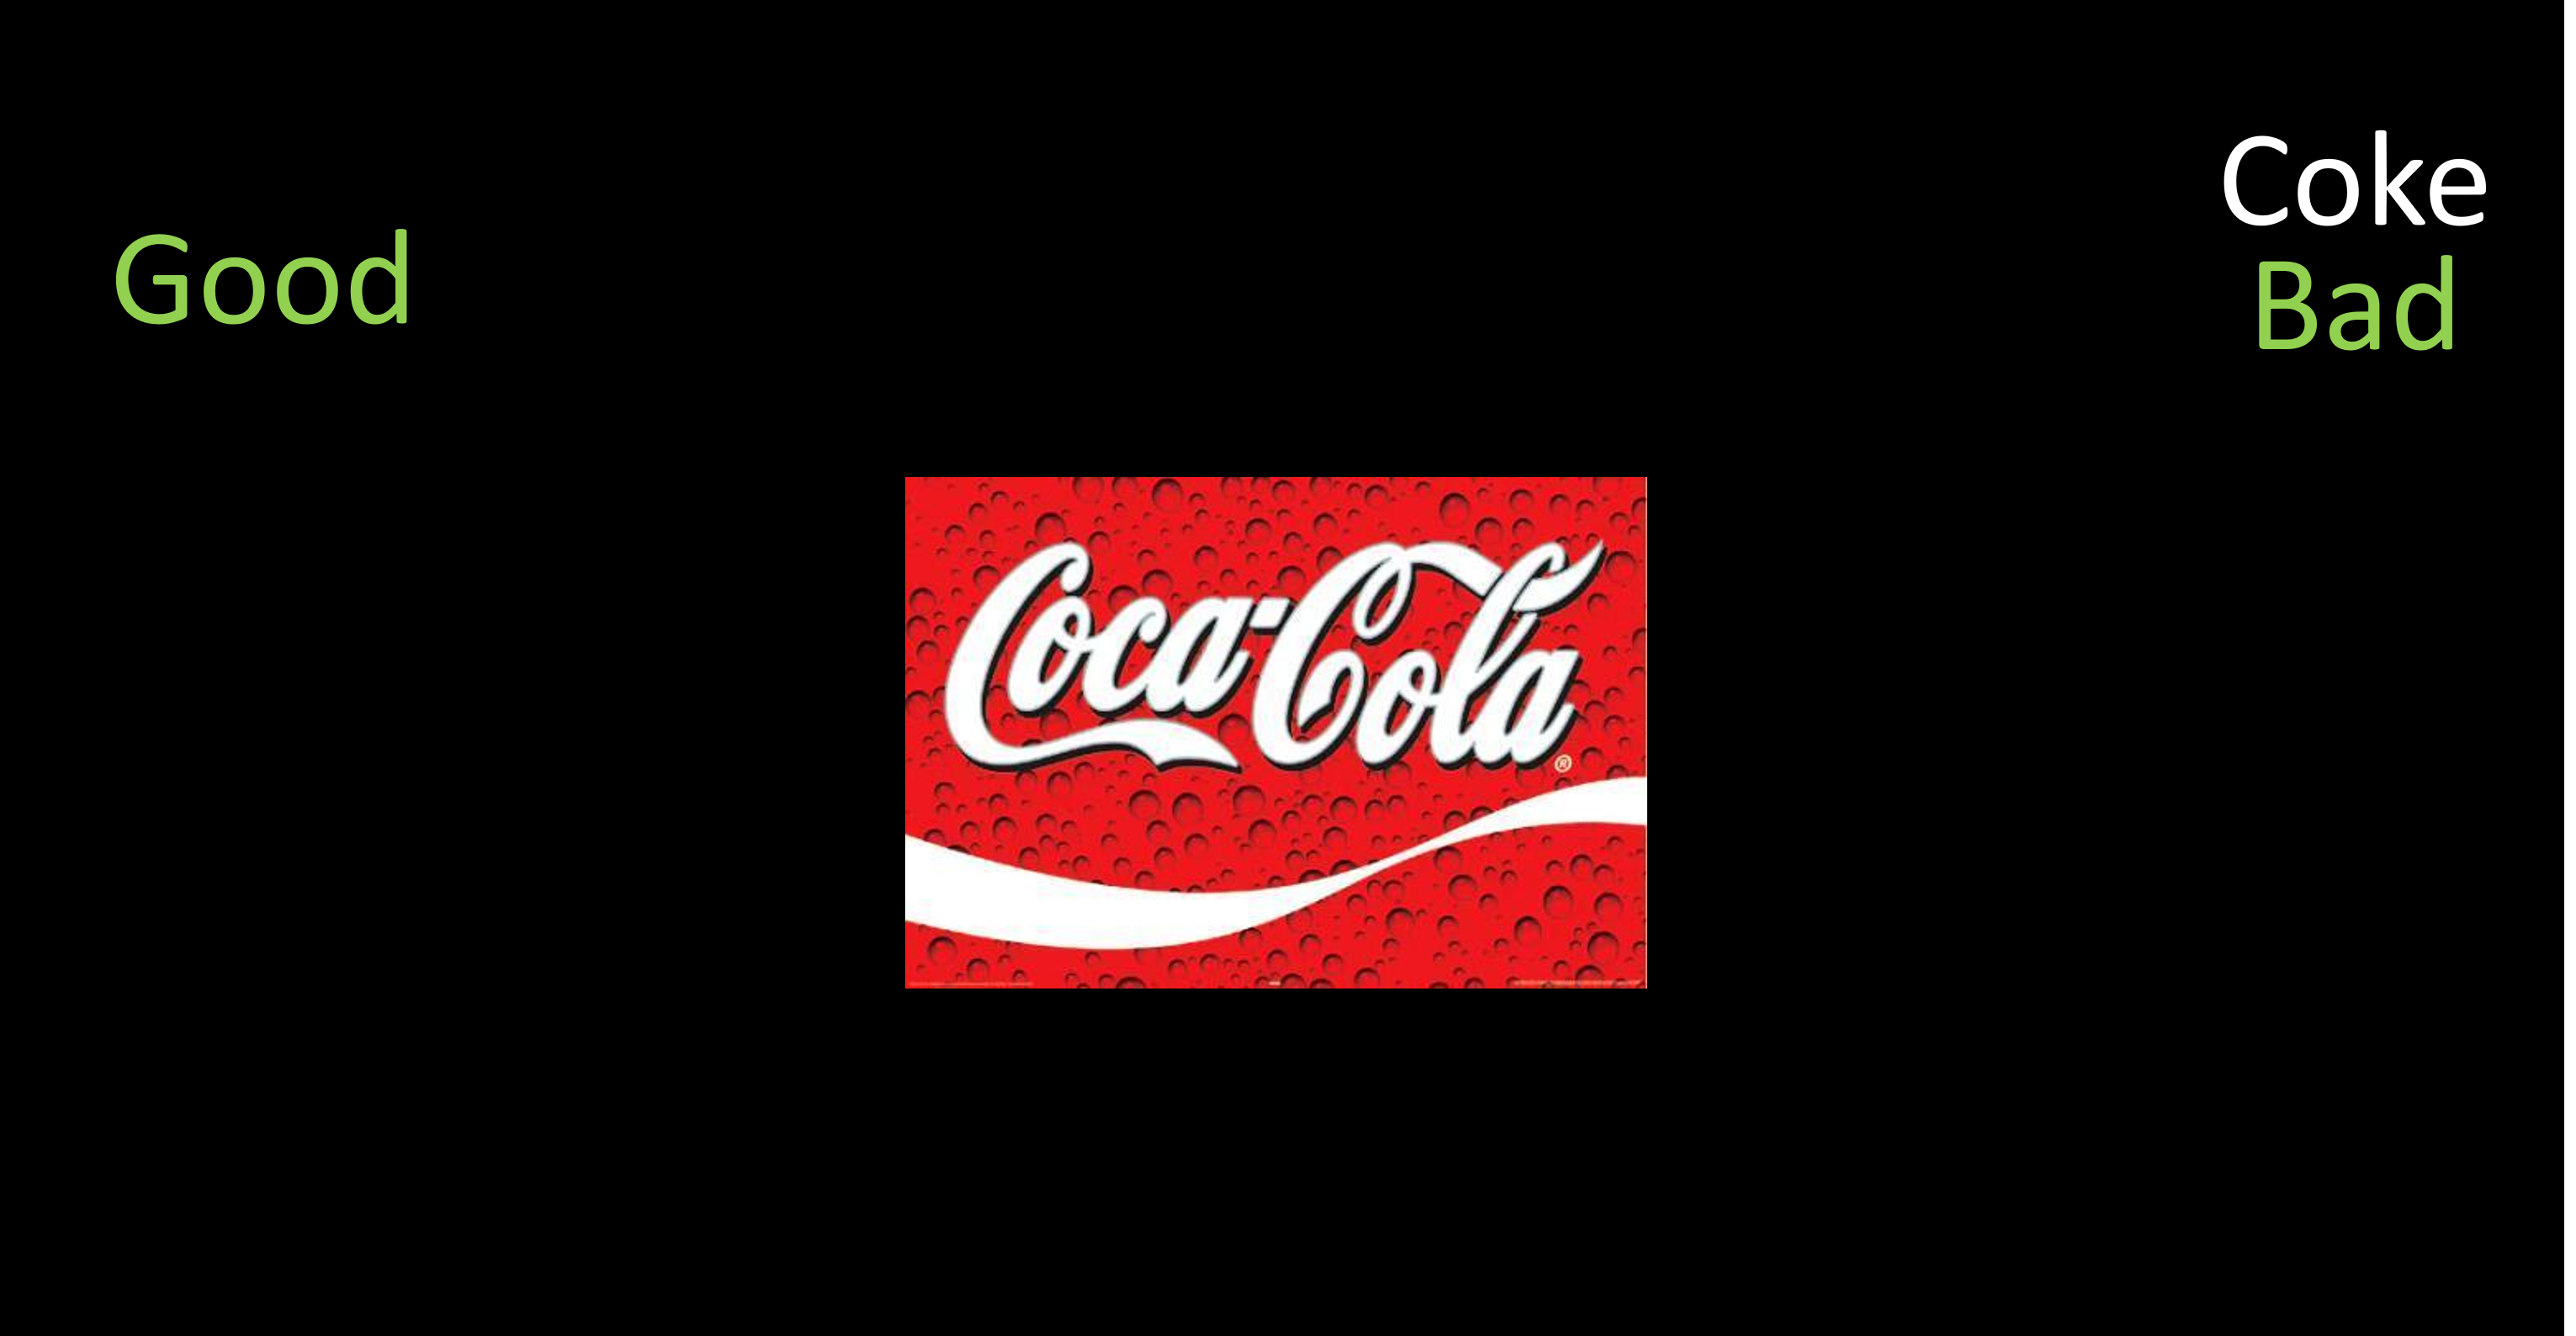
\includegraphics[width=\linewidth]{scBad.png}
		\end{figure}
	\end{columns}
	
\end{frame}


\begin{frame}{No Pepsi? No problem}
	\begin{columns}
		\column{.5\linewidth}
		\centering{\textcolor{unipd}{Pepsi-Good}}
		\begin{figure}
			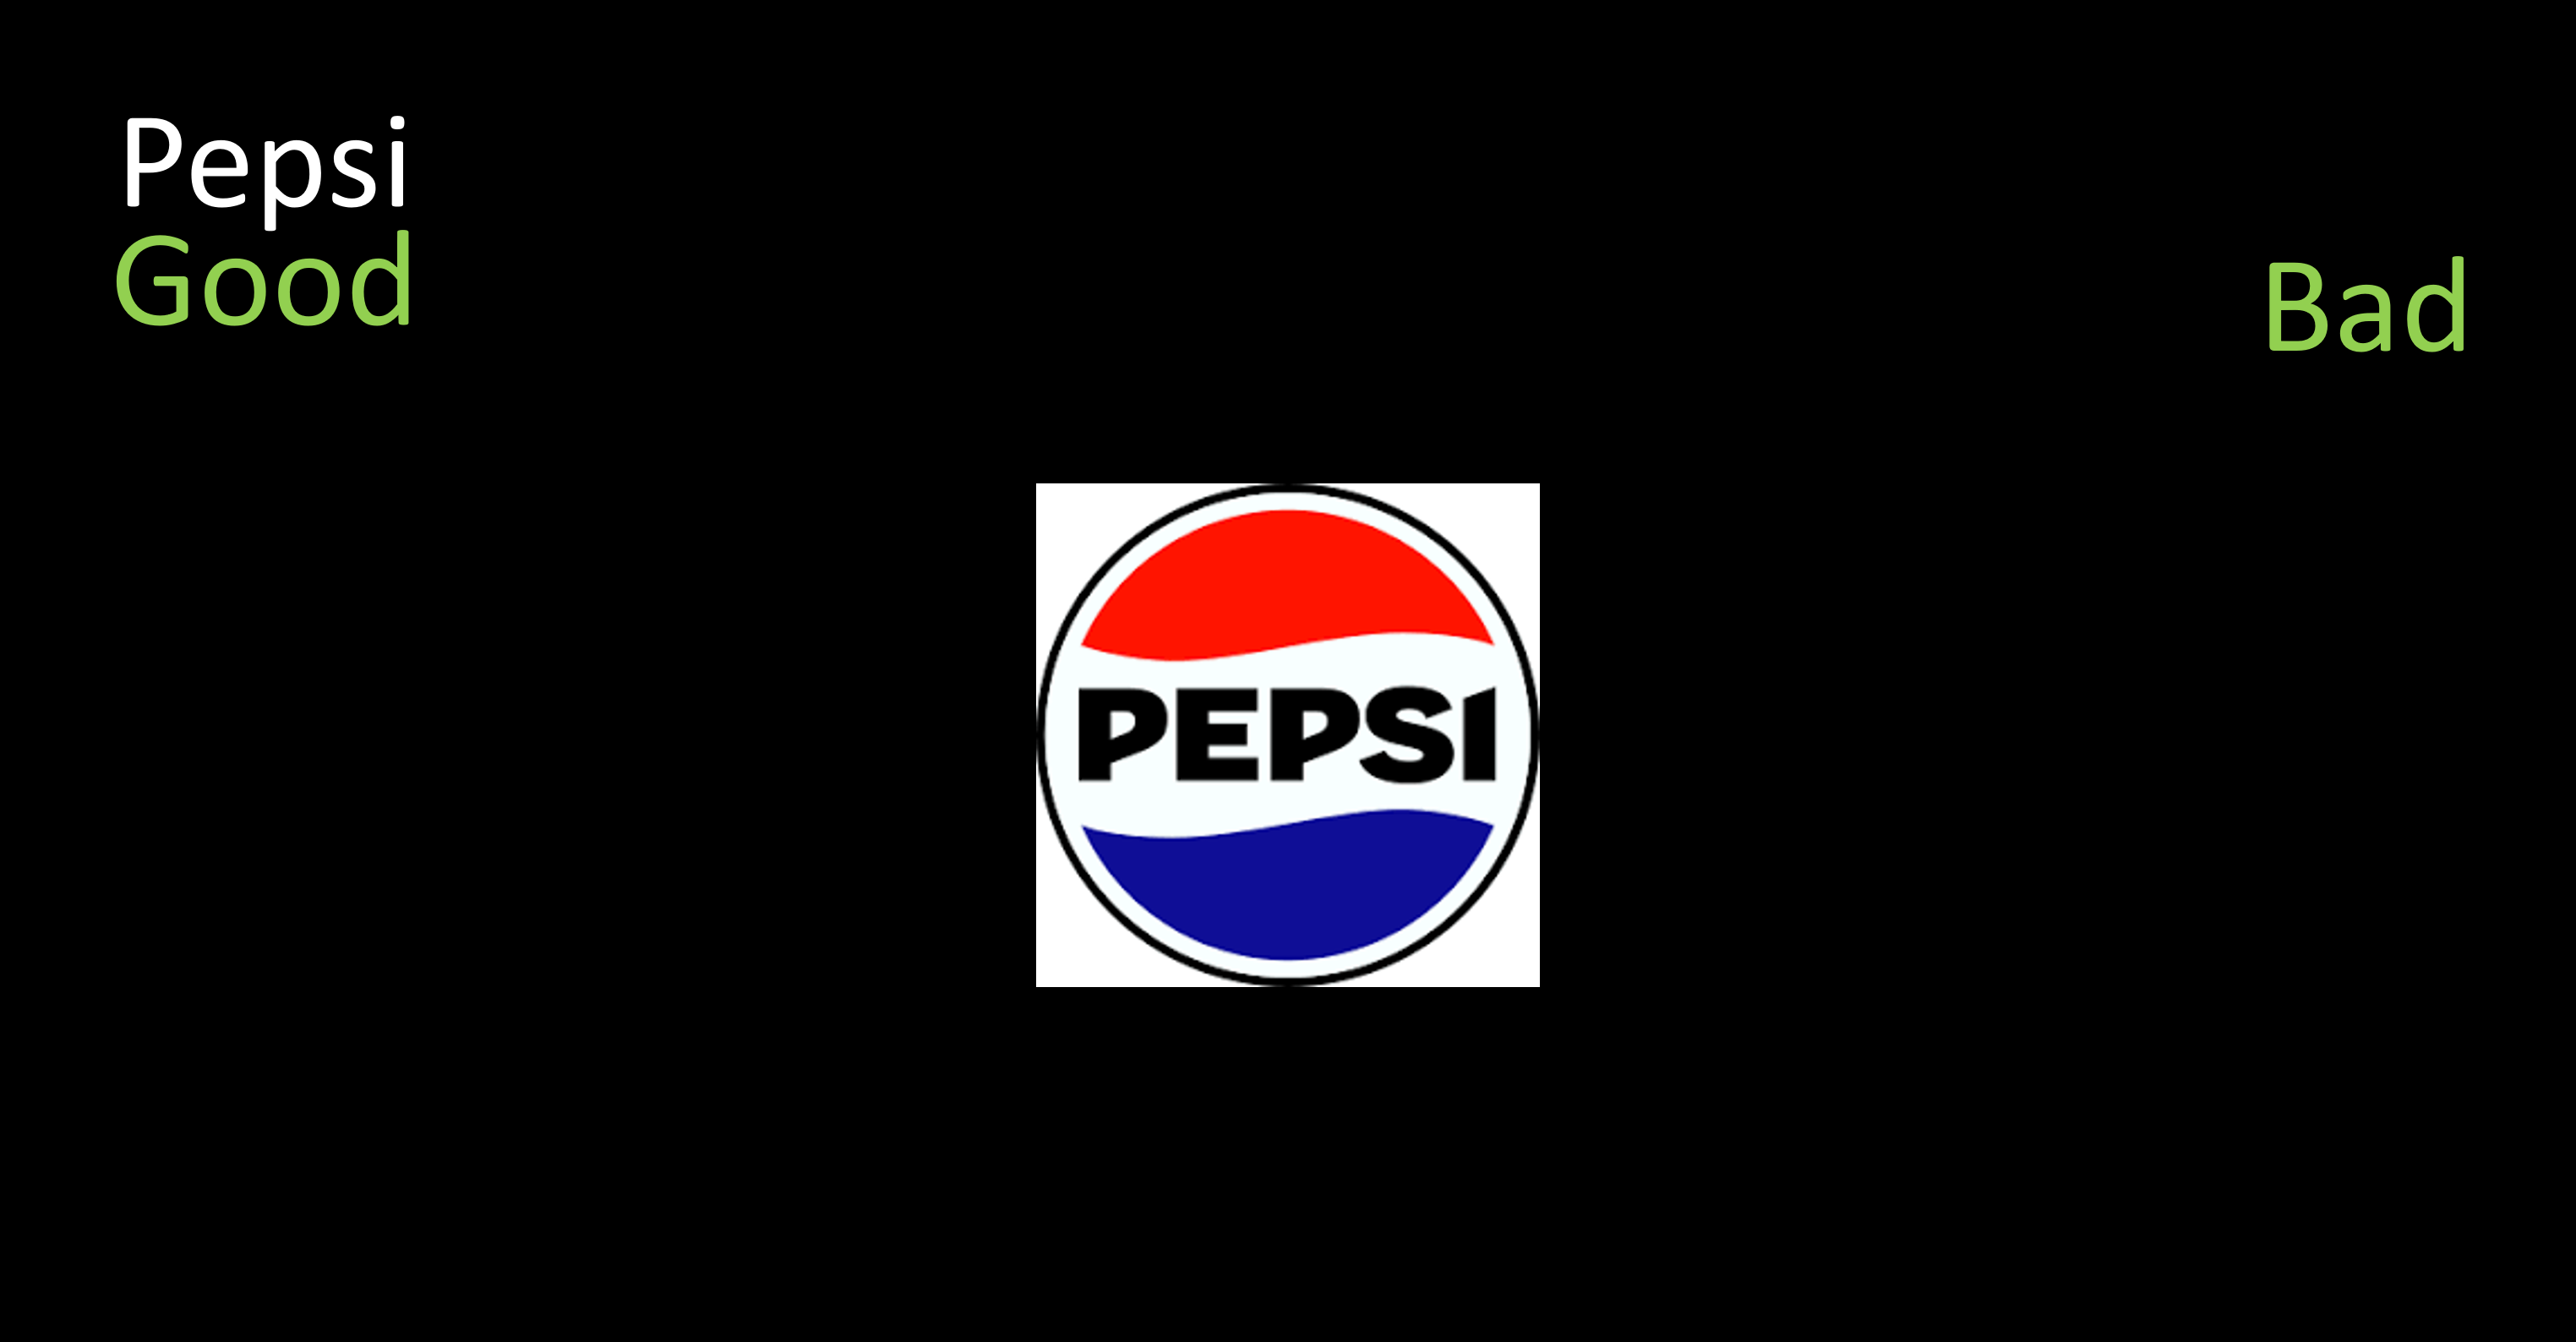
\includegraphics[width=\linewidth]{scPgood.png}
		\end{figure}
		
		\column{.5\linewidth}
		\centering{\textcolor{blu}{Pepsi-Bad}}
		\begin{figure}
			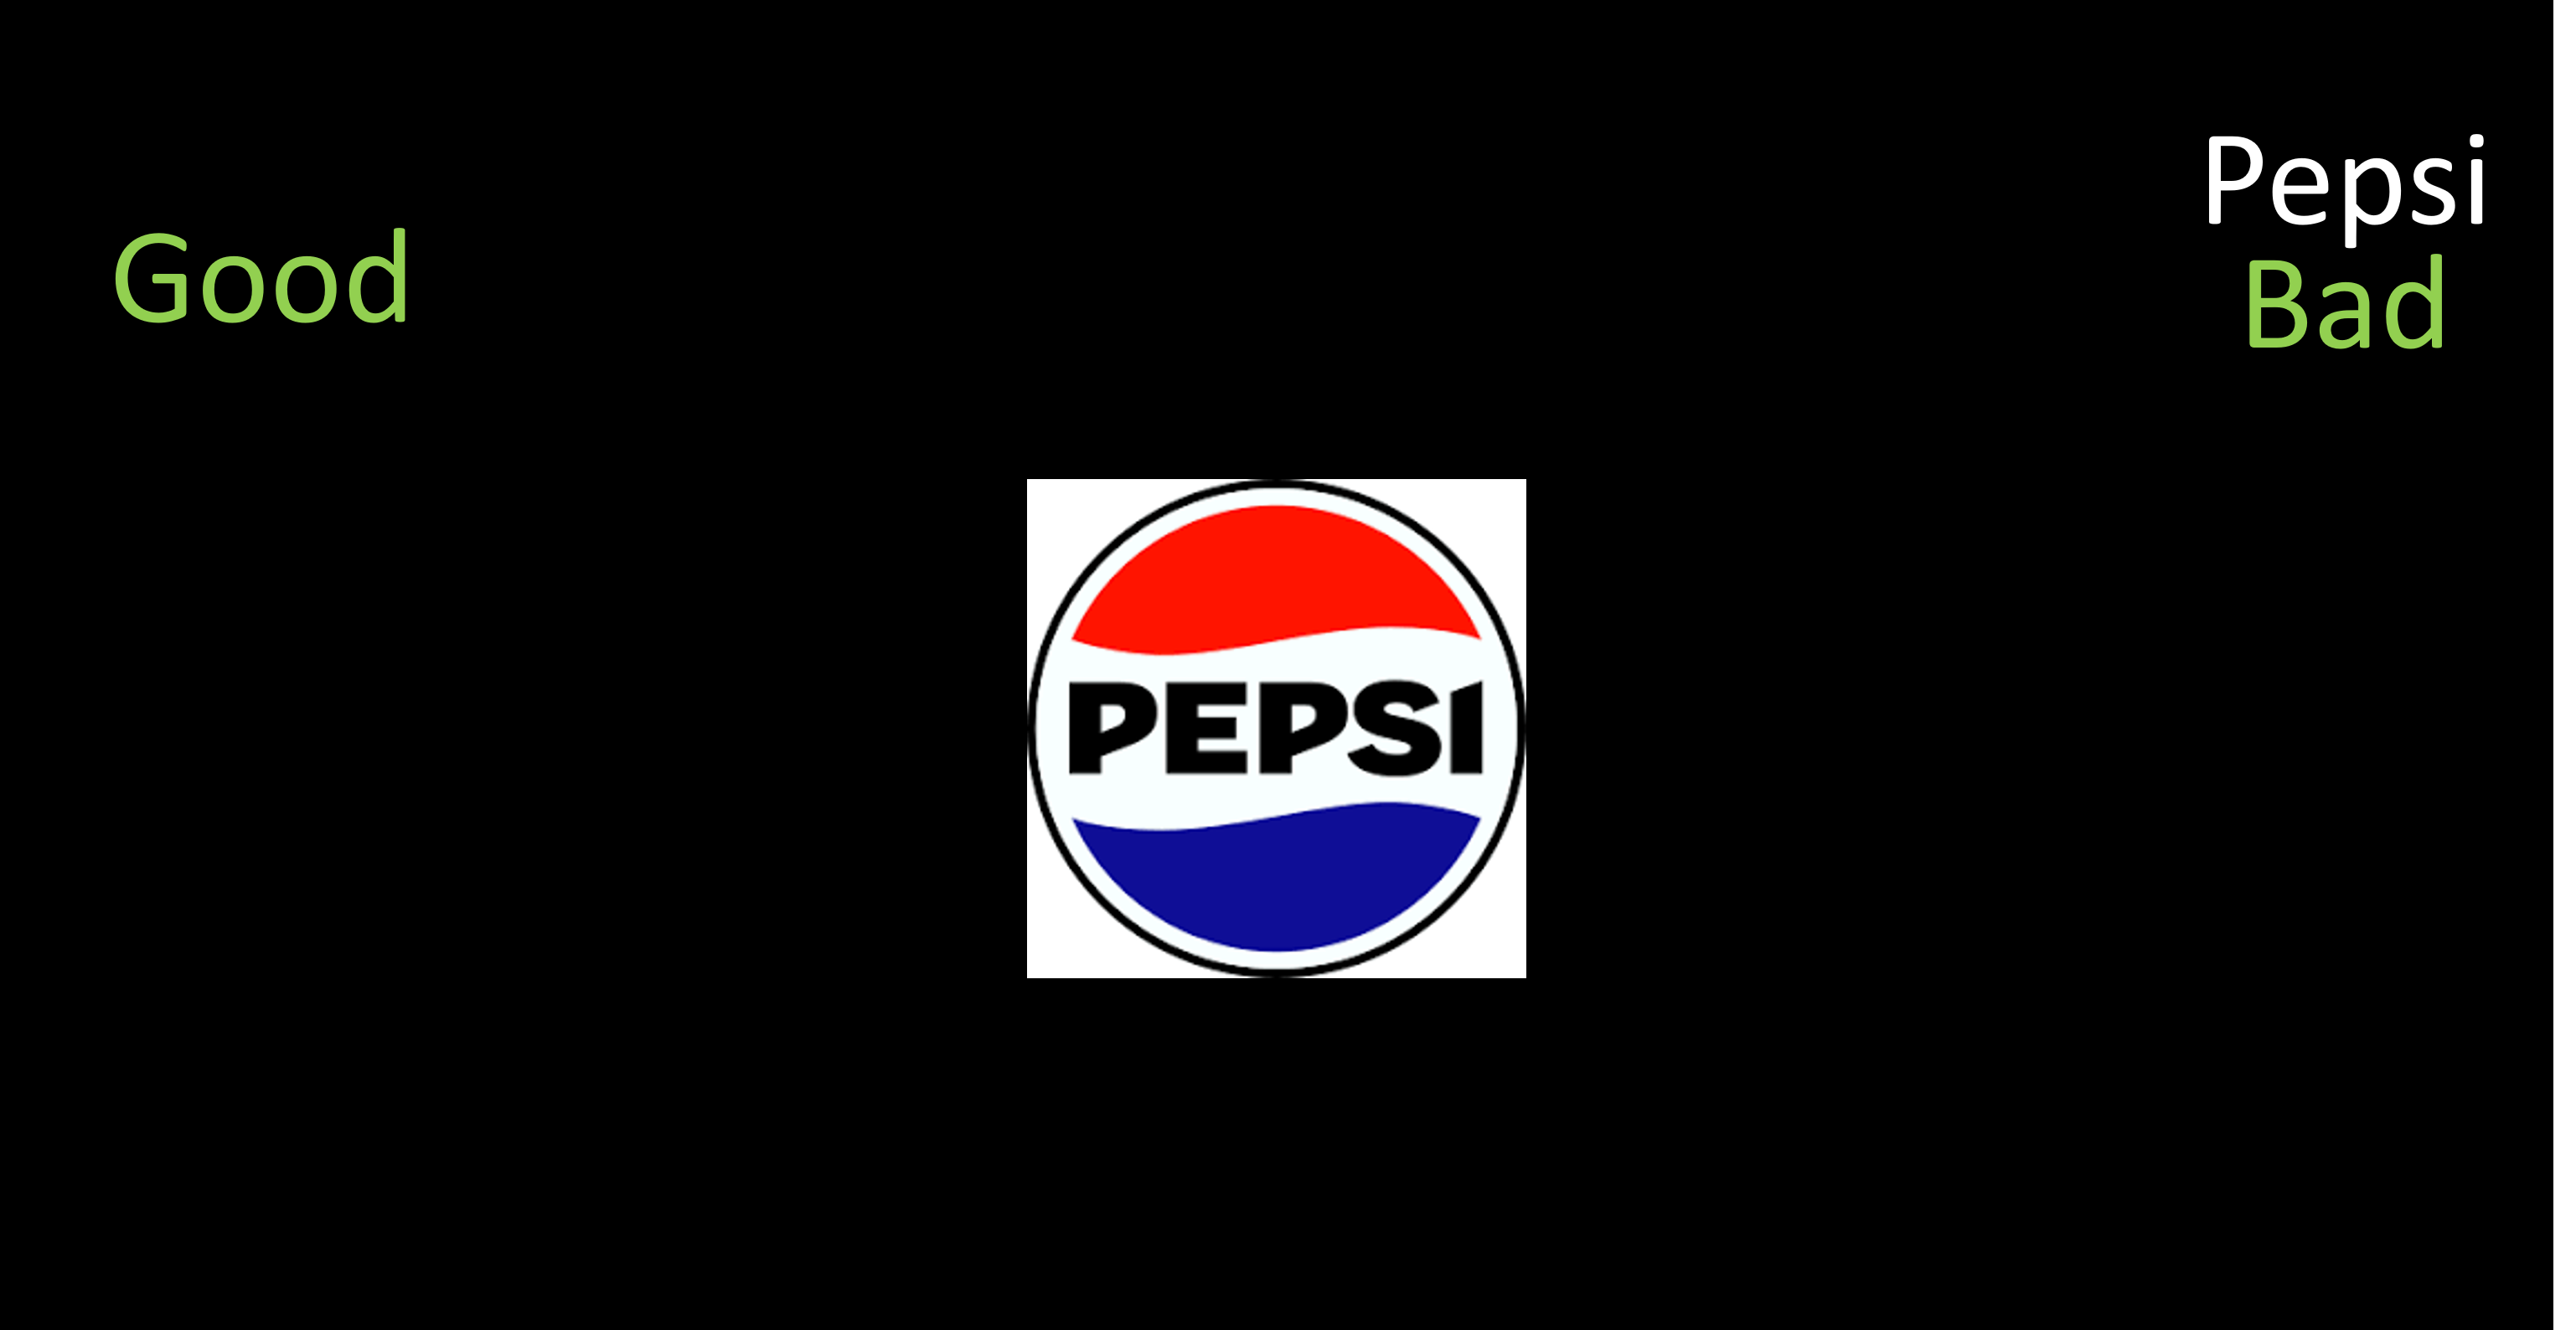
\includegraphics[width=\linewidth]{scPbad.png}
		\end{figure}
	\end{columns}
\end{frame}


\begin{frame}{Scoring}
	\vskip0pt plus 1filll
	\begin{equation*}
		D = \frac{M_{\mathrm{B2}} - M_{\mathrm{B4}}}{s_{\mathrm{B2, B4}}}
	\end{equation*}
	
	\vspace{5mm}
	
	\begin{itemize}
		\item Risposte $< 350$ms $ \rightarrow $ Eliminate
		\vspace{5mm}
		\item Risposte $> rtw$ $ \rightarrow $ Eliminate
		\vspace{5mm}
		\item Risposte errate $\rightarrow$ $M + 400$ms 
	\end{itemize}
	\vskip0pt plus 1filll
	
	\color{template}\rule{0.30\linewidth}{0.5pt}\\
	\color{black}
	\scriptsize{Karpinski, A., \& Steinman, R. B. (2006). The single
		category implicit association test as a measure of
		implicit social cognition.\emph{ Journal of Personality and
			Social Psychology, 91}(1), 16–32. https://doi.org/10
		.1037/0022-3514.91.1.16}
	
\end{frame}

\subsection{Go-No/Go Association Task}
\begin{frame}{Go-No/Go Association Task}{Nosek \& Banaji (2001)}

	
	
	\begin{table}
		\caption{GNAT}
		\begin{tabular}{c c c c }
			\hline
			Blocco	&	\# Trial	&	Signal (Spazio)	&	Noise (Niente)	\\
			\hline
			1	&	16	&	Good	&	Bad	\\
			2	&	16	&	Bad	&	Good	\\
			3	&	16	&	Fruit	&	Bugs	\\
			4	&	16	&	Bugs	&	Fruit	\\
			\hline
			\textcolor<2>{blu}{5}	&	\textcolor<2>{blu}{16}	&	\textcolor<2>{blu}{Good + Fruit}	&	\textcolor<2>{blu}{Bad + Bugs}	\\
			&	\textcolor<2>{blu}{60}	&	\textcolor<2>{blu}{Good + Fruit}	&	\textcolor<2>{blu}{Bad + Bugs}	\\
			\textcolor<2>{unipd}{6}	&	\textcolor<2>{unipd}{16}	&	\textcolor<2>{unipd}{Bad + Fruit}	&	\textcolor<2>{unipd}{Good + Bugs}	\\
			&	\textcolor<2>{unipd}{60}	&	\textcolor<2>{unipd}{Bad + Fruit}	&	\textcolor<2>{unipd}{Good + Bugs}	\\
			\hline
			\textcolor<3>{blu}{7}	&	\textcolor<3>{blu}{16}	&	\textcolor<3>{blu}{Good + Bugs}	&	\textcolor<3>{blu}{Bad + Fruit}	\\
			&	\textcolor<3>{blu}{60}	&	\textcolor<3>{blu}{Good + Bugs}	&	\textcolor<3>{blu}{Bad + Fruit}	\\
			\textcolor<3>{unipd}{8}	&	\textcolor<3>{unipd}{16}	&	\textcolor<3>{unipd}{Bad + Bugs}	&	\textcolor<3>{unipd}{Good + Fruit}	\\
			&	\textcolor<3>{unipd}{60}	&	\textcolor<3>{unipd}{Bad + Bugs}	&	\textcolor<3>{unipd}{Good + Fruit}	\\
			\hline
		\end{tabular}
	\end{table}
	
	
\end{frame}



\begin{frame}
	\vskip0pt plus 1filll
	
	\begin{columns}
		\column{.5\linewidth}
		\centering{\large{\textbf{\textcolor{green}{GO}}}}
		\begin{figure}
			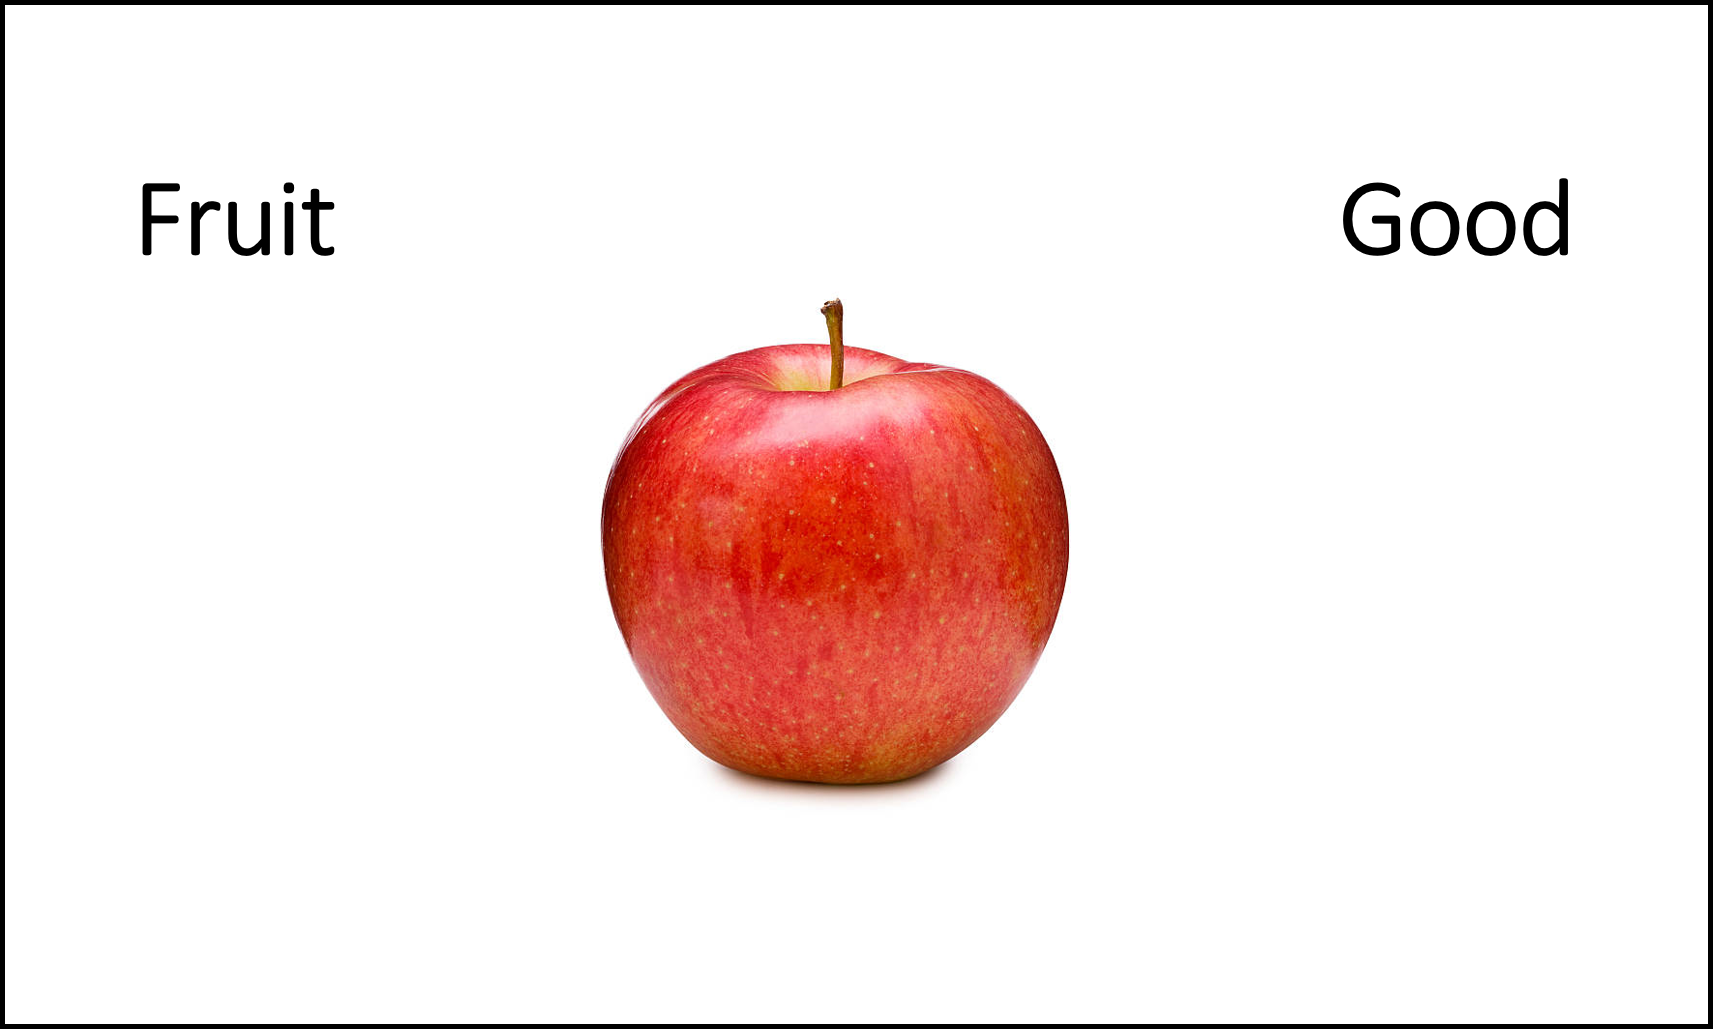
\includegraphics[width=\linewidth]{go.png}
		\end{figure}
		
		\column{.5\linewidth}
		\centering{\large{\textbf{\textcolor{unipd}{NO GO}}}}
		\begin{figure}
			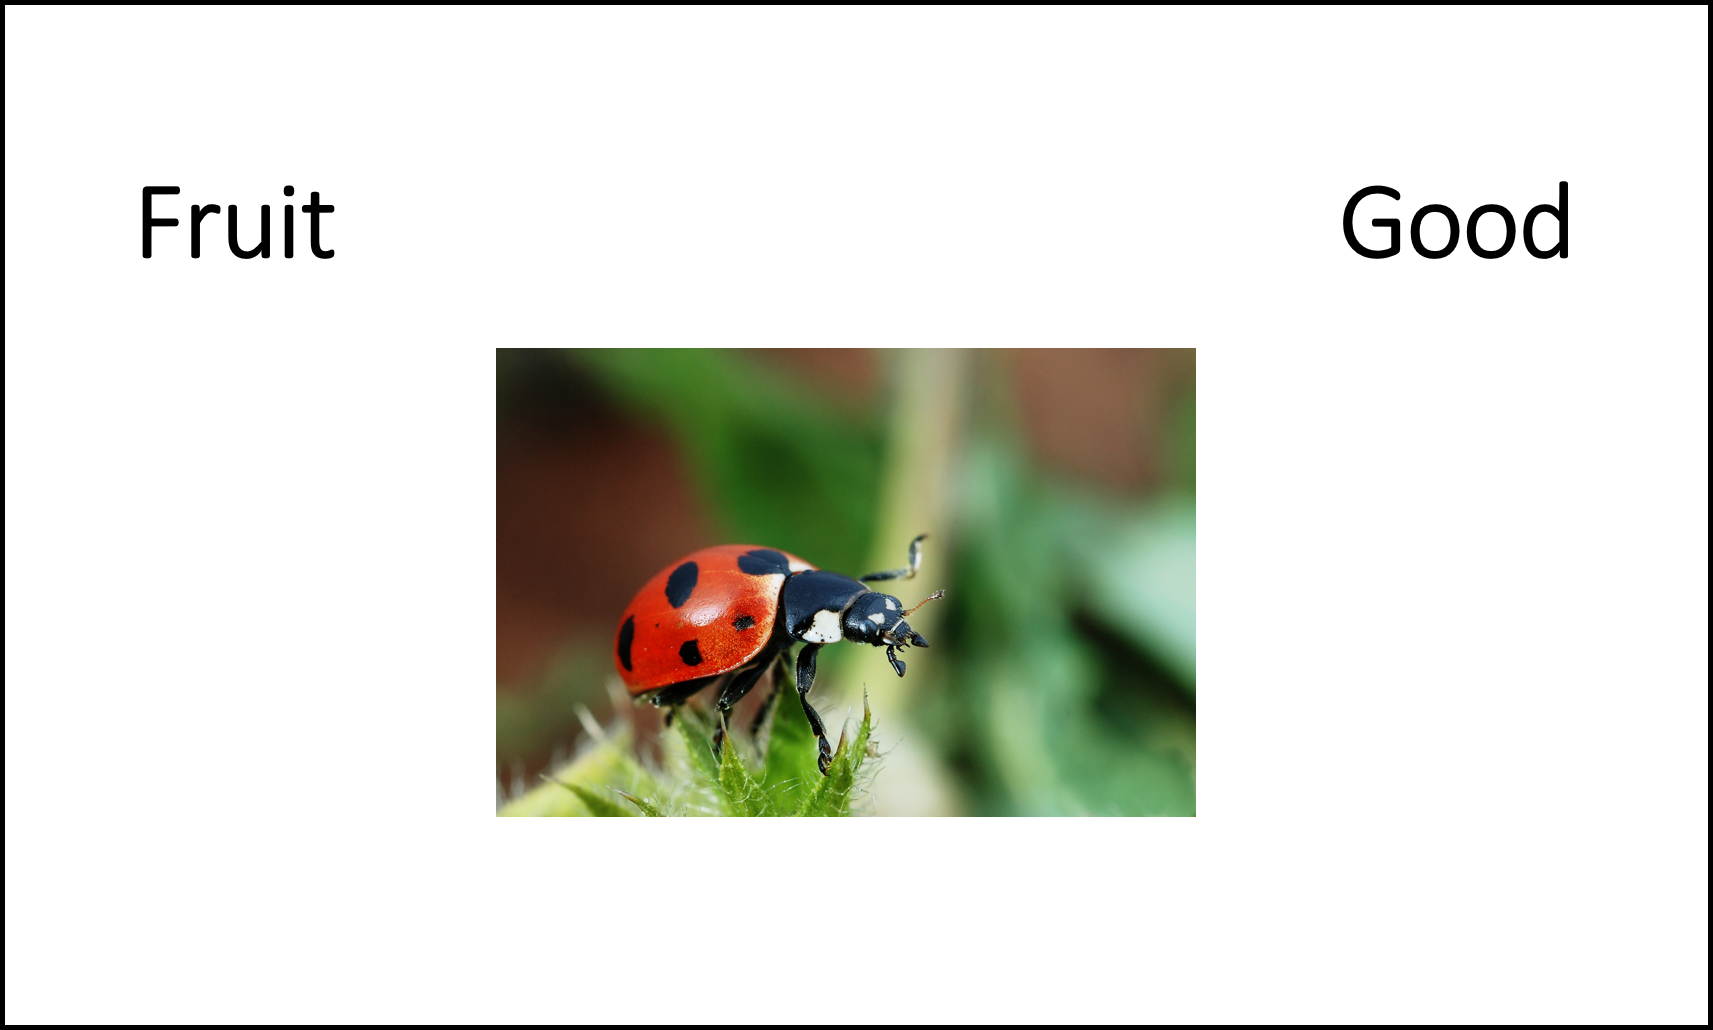
\includegraphics[width=\linewidth]{nogo.png}
		\end{figure}
	\end{columns}
	
	\vskip0pt plus 1filll
	
	
	\color{template}\rule{0.30\linewidth}{0.5pt}\\
	\color{black}
	
	\scriptsize{Nosek, B. A., \& Banaji, M. R. (2001). The go/no-go
		association task. \emph{Social Cognition, 19}(6), 625–666.
		Q21 https://doi.org/10.1521/soco.19.6.625.20886}
\end{frame}

\begin{frame}{Scoring}
	
	$ d' $ (Green \& Swets, 1966): 
	
	\vspace{5mm}
	
	\begin{enumerate}
		\item Standardizzazione della proporzione di ``hits'' (risposte ``go'' in presenza del segnale)  
		\item Standardizzazione della proporzione di ``false alarms'' (risposte ``go'' in presenza di rumore)
		\item Differenza tra i due punteggi
	\end{enumerate}
	
	%	\vspace{5mm}
	%	
	%	Empty cells (no false alarms or misses) $\rightarrow$ $0.35/\mathrm{number \, of \, trials}$
\end{frame}

\subsection{Sorting Paired Features Task}
\begin{frame}{Sorting Paired Features Task}
	\vskip0pt plus 1filll
	Bar-Anan et. al (2009):
	
	\begin{footnotesize}
		\begin{spacing}\Factor
			\begin{table}
				\centering
				\caption{SPF}
				\begin{tabular}{c c c c c c}
					\hline
					Blocks	&	Trials	&	Top-left	&	Top-right	&	Bottom-left	&	Bottom-right	\\
					\hline
					1	&	48	&	Dogs+Good	&	Dogs+Bad	&	Cats+Good	&	Cats+Bad	\\
					2	&	48	&	Dogs+Bad	&	Dogs+Good	&	Cats+Bad	&	Cats+Good	\\
					3	&	48	&	Cats+Bad	&	Cats+Good	&	Dogs+Bad	&	Dogs+Good	\\
					4	&	48	&	Cats+Good	&	Cats+Bad	&	Dogs+Good	&	Dogs+Bad	\\
					\hline
					
				\end{tabular}
			\end{table}
		\end{spacing}
	\end{footnotesize}
	
	\vspace{3mm}
	
	Viene associata una chiave di risposta della tastiera ad ognuno dei possibili pairing 
	
	\vskip0pt plus 1filll
	
	\color{template}\rule{0.30\linewidth}{0.5pt}\\
	\color{black}
	\scriptsize{Bar-Anan, Y., Nosek, B. A., \& Vianello, M. (2009).
		The sorting paired features task: A measure of
		association strengths. \emph{Experimental Psychology,
			56}(5), 329–343. https://doi.org/10.1027/1618-3169.
		56.5.329}
\end{frame}

\begin{frame}
	\begin{columns}
		\column{.5\linewidth}
		\centering{\large{Correct key: M}}
		\begin{figure}
			
\includegraphics[width=\linewidth]{spf1.png}
		\end{figure}
		
		\column{.5\linewidth}
		\centering{\large{\large{Correct key: P}}}
		\begin{figure}
			
\includegraphics[width=\linewidth]{spf2.png}
		\end{figure}
	\end{columns}
\end{frame}


\section[Priming]{Misure implicite basate sul priming}


\begin{frame}{Procedure di priming}
	
	Vanno ad investigare l'associazione tra due stimoli presupponendo che il primo degli stimoli presentati (il \emph{prime}) abbia un effetto sulla percezione del secondo stimolo (il \emph{target})
	
	\vspace{1.5mm}
	La presentazione del prime è estremamente veloce (pochi millesimi di secondo), quasi non ci si accorge che viene presentato
	
	\vspace{1.5mm}
	La presentazione del target avviene a velocità ``normale''
	
	\vspace{1.5mm}
	Ci si aspetta che se i due stimoli sono effettivamente associati tra loro per la persona, questa impiegherà meno tempo a dare una risposta al target quando questo è associato al prime piuttosto che quando non lo è 
	
\end{frame}

\begin{frame}
	\begin{figure}
		\centering
		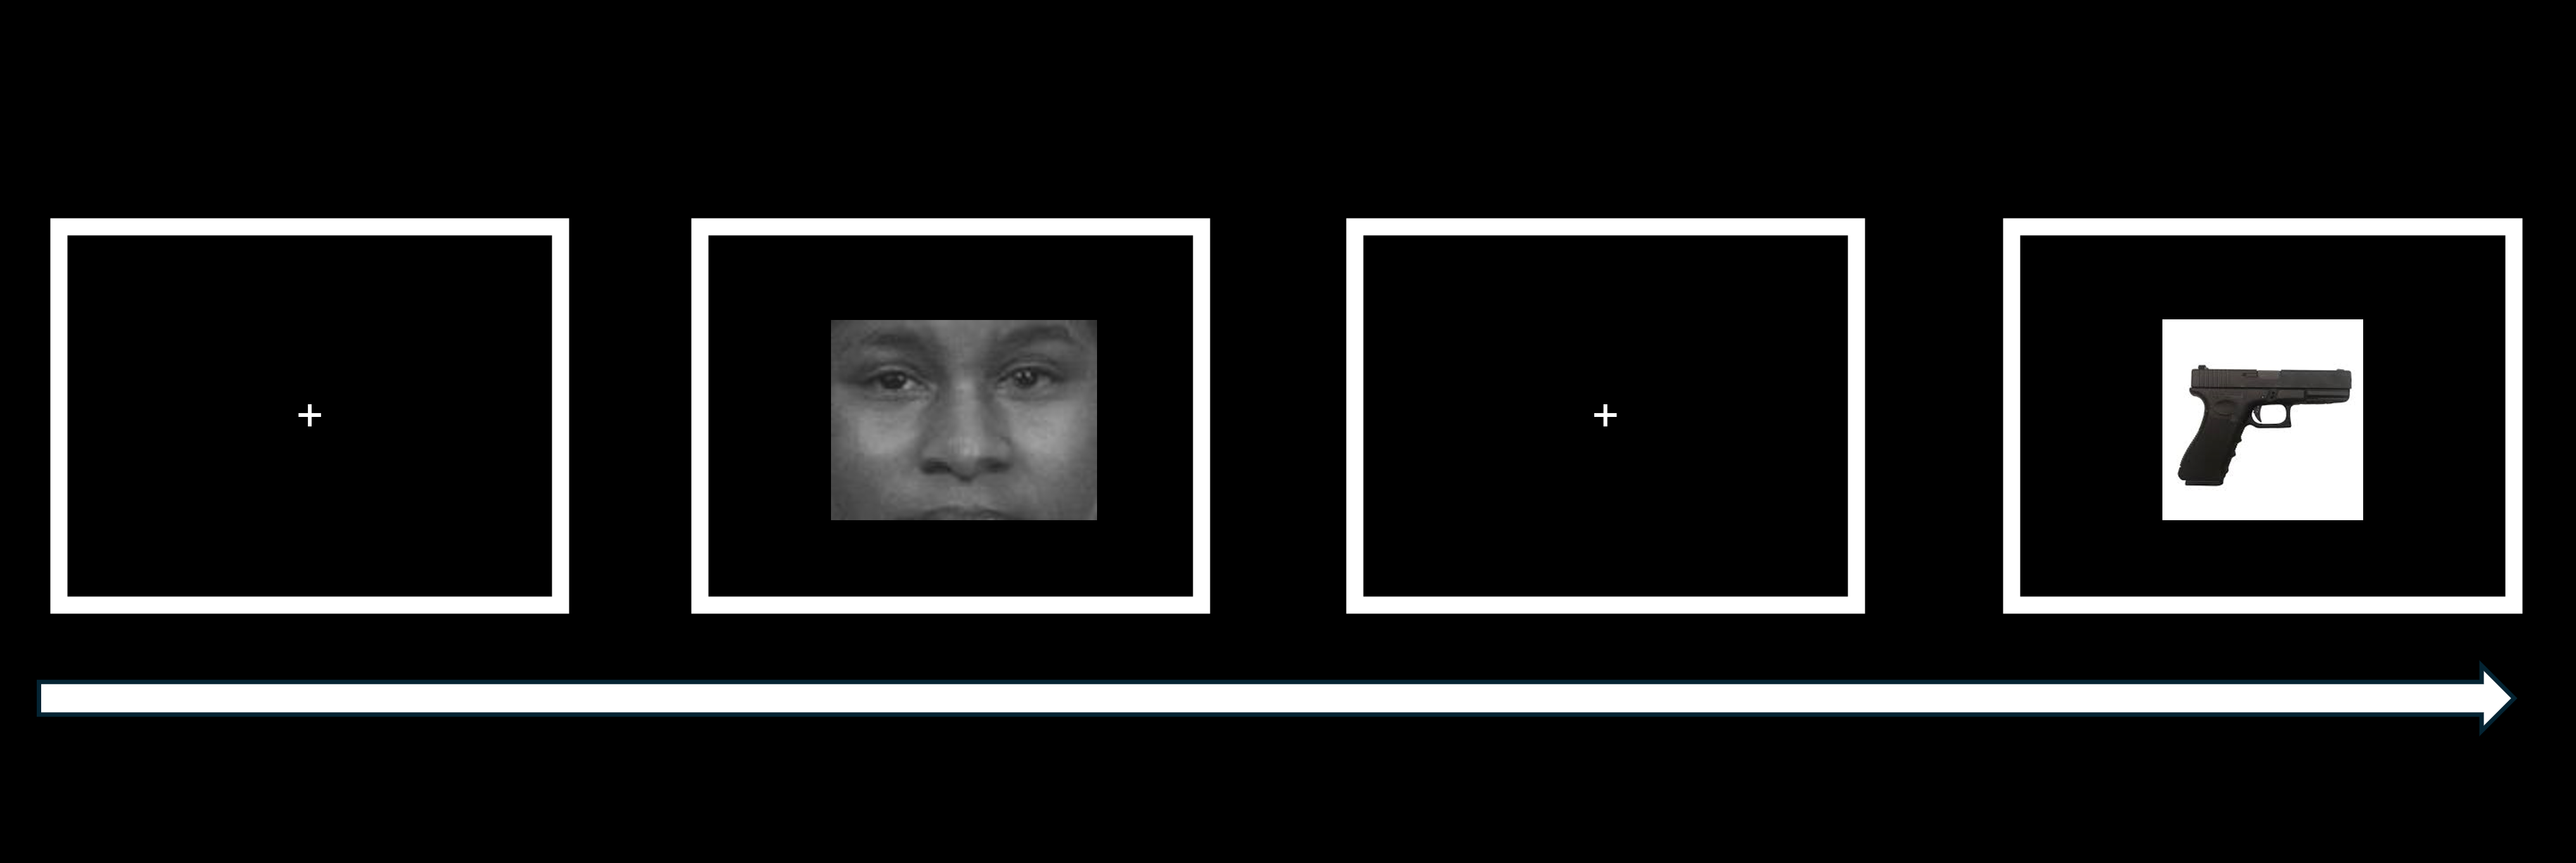
\includegraphics[width=\linewidth]{prime}
	\end{figure}
	
	Se una persona impiega meno tempo e commette meno errori a riconoscere la pistola quando questa è preceduta da una persona Nera piuttosto che da una persona Bianca $\rightarrow$ possibile pregiudizio nei confronti delle persone Nere
\end{frame}

\subsection{Affective Misattribution Procedure}

\begin{frame}
	
	\begin{figure}
		\centering
		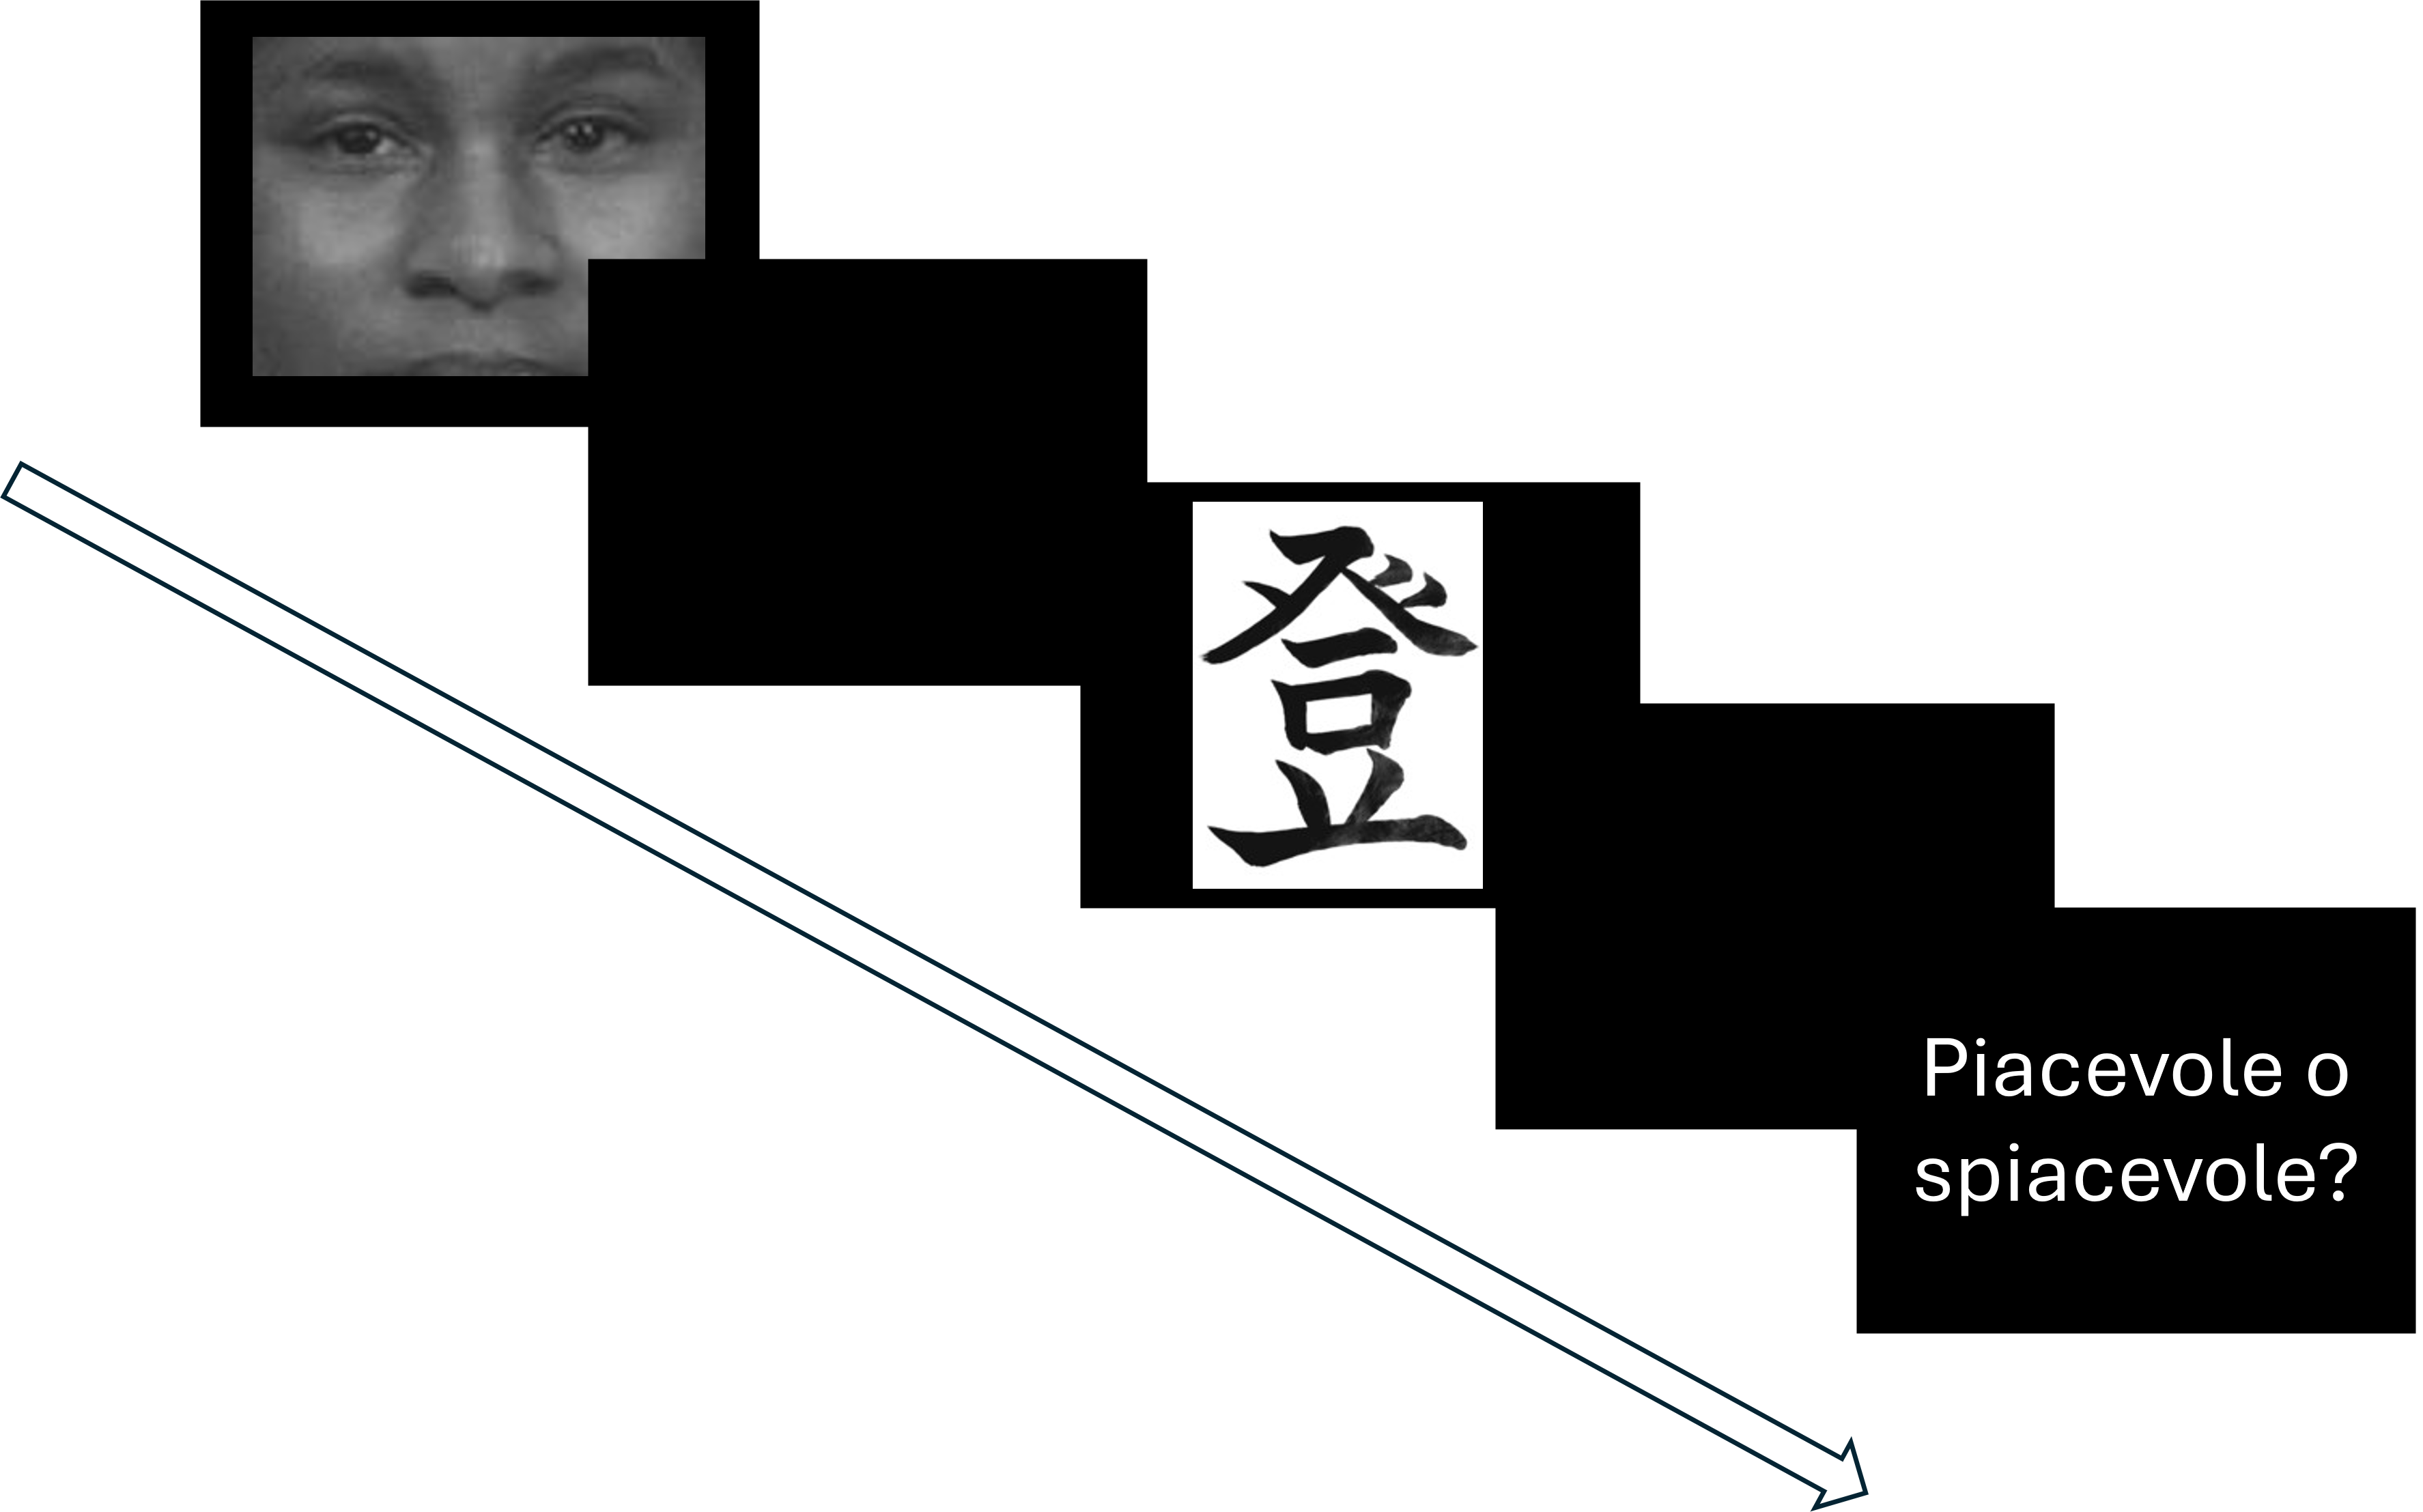
\includegraphics[width=.7\linewidth]{AMP}
	\end{figure}
	
	
	\vskip0pt plus 1filll
	
	
	\color{template}\rule{0.30\linewidth}{0.5pt}\\
	\color{black}
	
	\scriptsize{Payne, B. K., Cheng, C. M., Govorun, O., \& Stewart, B. D. (2005). An inkblot for attitudes: affect misattribution as implicit measurement. \emph{Journal of Personality and Social Psychology, 89}(3), 277. https://doi.org/10.1037/0022-3514.89.3.277}
\end{frame}



\begin{frame}
	\begin{center}
	
\includegraphics[width=.20\linewidth]{work.png}
\end{center}

Pensare (in gruppo) a uno o più argomenti di indagine: 

\begin{itemize}
	\item Quale tecnica si presta meglio tra associazioni automatiche e tecniche di priming?
	
	\item Come strutturereste l'esperimento? con quali categorie? con che tipologia di stimoli?
	
	\item Sarebbe lo stesso processo per l'indagine di temi di cognizione sociale e altri temi?
\end{itemize}
\end{frame}

\section{A measure in search of a construct}

\begin{frame}{Cosa misura lo IAT?}
	
	
	
	\begin{enumerate}
		\item Lo IAT non è una misura valida per lo studio delle \emph{caratteristiche di personalità} perché non ci sono caratteristiche di personalità stabili che influenzano davvero la performance allo IAT
		\pause
		\item In realtà queste caratteristiche ci sono... solo lo IAT non lo le riesce a misurare!
			\pause
		\item In realtà, lo IAT misura queste caratteristiche, lo fa bene,  però si possono misurare anche con le misure esplicite!
			\pause
		\item In realtà, lo IAT è effettivamente una misura di costrutti che non possono essere misurati con le misure esplicite
	\end{enumerate}
	
\end{frame}

\begin{frame}{Differenze individuali?!}
\begin{figure}
	\centering
	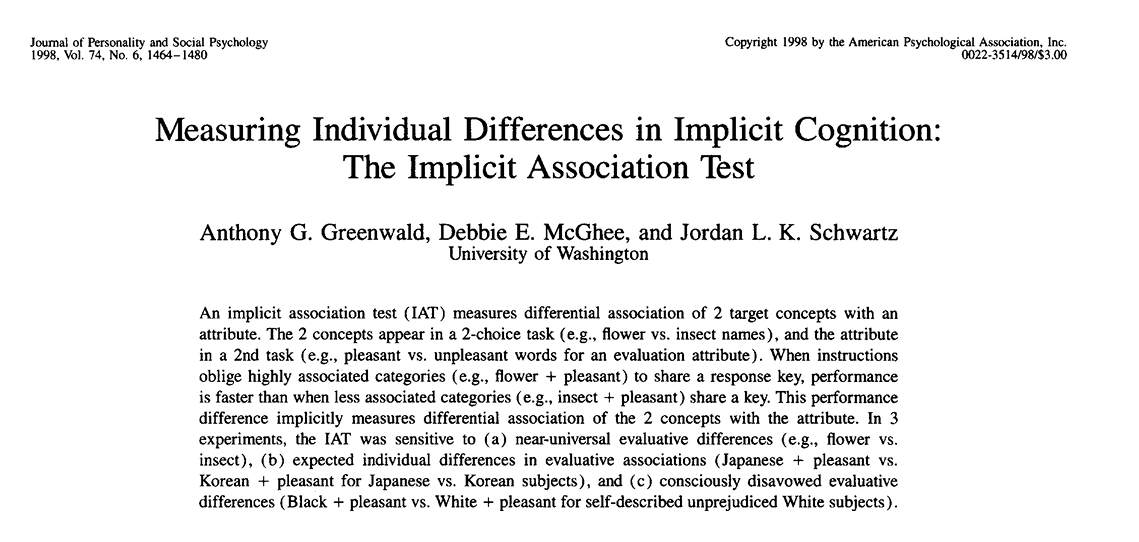
\includegraphics[width=\linewidth]{iat-pub}
\end{figure}

\end{frame}

\begin{frame}
	IAT come misura della forza di associazioni relative \underline{a livello di gruppo}
	
	\vspace{1.5mm}
	\begin{quote}
		Non c'è dubbio sulla sua validità per fare questo!
	\end{quote}
	
	\pause
	\vspace{1.5mm}
	
	Il problema è che lo IAT è stato sviluppato con uno scopo differente... come misura delle \emph{differenze individuali}!
	
	\pause 
	\vspace{1.5mm}
	
	Il fatto che lo IAT produca delle differenza di gruppo attendibili nella forza delle associazioni automatiche  \textbf{non implica} che produca misure valide delle differenze individuali
	
	
\end{frame}

\begin{frame}{Quali conseguenze}
	\begin{itemize}
		\item Scarsa correlazione con le misure esplicite
		\vspace{1.5mm}
		\item Scarsa capacità predittiva dei comportamenti osservati 
	\end{itemize}
	
	\pause
\begin{center}
C'è un però
\end{center}

\begin{itemize}
	\item La misura dello IAT correla con le misure esplicite in ambiti non socialmente rilevanti 
	\item Il tipo di comportamento (intenzionale vs. non intenzionale) considerato negli studi 
\end{itemize}

\vskip0pt plus 1filll

\color{template}\rule{0.30\linewidth}{0.5pt}\\
\color{black}
\footnotesize{Carlsson, R., \& Agerstrom, J. (2016). A closer look at the discrimination outcomes in the IAT literature. \emph{Scandinavian Journal of Psychology, 57}(4), 278–287. doi:
	https://doi.org/10.1111/sjop.12288\\
	Schimmack, U. (2021). The Implicit Association Test:
	A method in search of a construct. \emph{Perspectives on
		Psychological Science, 16}(2), 396–414. https://
	doi.org/10.1177/1745691619863798}
\end{frame}


\begin{frame}{Uno dei problemi}{Il metodo di scoring}
		\begin{spacing}\Factor
		\begin{table}[th!]
			\scalebox{.9}{
			\begin{tabular}{llll}
				\hline
				\emph{D score} & Risposte errate & Risposte troppo veloci\\\hline
				\emph{D1} & Built-in correction & No \\
				\emph{D2} & Built-in correction & Eliminare trials $<$ 400 \emph{ms} \\
				\emph{D3} & Mean (correct responses) + 2\emph{sd} & No\\
				\emph{D4} & Mean (correct responses) + 600 \emph{ms} & No \\
				\emph{D5} & Mean (correct responses) + 2\emph{sd} & Eliminare trials $<$ 400 \emph{ms}\\
				\emph{D6} & Mean (correct responses) + 600 \emph{ms} & Eliminare trials $<$ 400 \emph{ms} \\\hline
			\end{tabular}
			}
			
		\end{table}
	\end{spacing}
	
	L'algoritmo di scoring usato... è spesso un mistero!
	
	Inoltre, la struttura dei dati dello IAT non si presta molto al calcolo di un indice semplice come il \emph{D} score
	
 
\end{frame}


%\begin{frame}{Alcuni dei problemi}
%	\begin{itemize}
%		\item La presenza di diversi scoring senza alcuna indicazione su quale usare e quando 
%		\item La presentazione del feedback 
%	\end{itemize}
%\end{frame}



\end{document}